%% bare_conf.tex
%% V1.3
%% 2007/01/11
%% by Michael Shell
%% See:
%% http://www.michaelshell.org/
%% for current contact information.
%%
%% This is a skeleton file demonstrating the use of IEEEtran.cls
%% (requires IEEEtran.cls version 1.7 or later) with an IEEE conference paper.
%%
%% Support sites:
%% http://www.michaelshell.org/tex/ieeetran/
%% http://www.ctan.org/tex-archive/macros/latex/contrib/IEEEtran/
%% and
%% http://www.ieee.org/

%%*************************************************************************
%% Legal Notice:
%% This code is offered as-is without any warranty either expressed or
%% implied; without even the implied warranty of MERCHANTABILITY or
%% FITNESS FOR A PARTICULAR PURPOSE! 
%% User assumes all risk.
%% In no event shall IEEE or any contributor to this code be liable for
%% any damages or losses, including, but not limited to, incidental,
%% consequential, or any other damages, resulting from the use or misuse
%% of any information contained here.
%%
%% All comments are the opinions of their respective authors and are not
%% necessarily endorsed by the IEEE.
%%
%% This work is distributed under the LaTeX Project Public License (LPPL)
%% ( http://www.latex-project.org/ ) version 1.3, and may be freely used,
%% distributed and modified. A copy of the LPPL, version 1.3, is included
%% in the base LaTeX documentation of all distributions of LaTeX released
%% 2003/12/01 or later.
%% Retain all contribution notices and credits.
%% ** Modified files should be clearly indicated as such, including  **
%% ** renaming them and changing author support contact information. **
%%
%% File list of work: IEEEtran.cls, IEEEtran_HOWTO.pdf, bare_adv.tex,
%%                    bare_conf.tex, bare_jrnl.tex, bare_jrnl_compsoc.tex
%%*************************************************************************

% *** Authors should verify (and, if needed, correct) their LaTeX system  ***
% *** with the testflow diagnostic prior to trusting their LaTeX platform ***
% *** with production work. IEEE's font choices can trigger bugs that do  ***
% *** not appear when using other class files.                            ***
% The testflow support page is at:
% http://www.michaelshell.org/tex/testflow/



% Note that the a4paper option is mainly intended so that authors in
% countries using A4 can easily print to A4 and see how their papers will
% look in print - the typesetting of the document will not typically be
% affected with changes in paper size (but the bottom and side margins will).
% Use the testflow package mentioned above to verify correct handling of
% both paper sizes by the user's LaTeX system.
%
% Also note that the "draftcls" or "draftclsnofoot", not "draft", option
% should be used if it is desired that the figures are to be displayed in
% draft mode.
%
\documentclass[conference]{IEEEtran}
% Add the compsoc option for Computer Society conferences.
%
% If IEEEtran.cls has not been installed into the LaTeX system files,
% manually specify the path to it like:
% \documentclass[conference]{../sty/IEEEtran}


% Some very useful LaTeX packages include:
% (uncomment the ones you want to load)
\usepackage{graphicx}
\usepackage{amssymb}
\usepackage[noadjust]{cite}
\usepackage{filecontents}
\usepackage[parfill]{parskip}
\usepackage[font=footnotesize]{subcaption}
\usepackage{hyperref}
\usepackage{url}
\usepackage{booktabs}
\usepackage[normalem]{ulem}
\usepackage[T1]{fontenc}
\renewcommand{\vec}[1]{\mathbf{#1}}
\usepackage{comment}
\usepackage{color}
\definecolor{indiagreen}{rgb}{0.07, 0.53, 0.03}

% *** GRAPHICS RELATED PACKAGES ***
%
%\ifCLASSINFOpdf
  % \usepackage[pdftex]{graphicx}
  % declare the path(s) where your graphic files are
  % \graphicspath{{../pdf/}{../jpeg/}}
  % and their extensions so you won't have to specify these with
  % every instance of \includegraphics
  % \DeclareGraphicsExtensions{.pdf,.jpeg,.png}
%\else
  % or other class option (dvipsone, dvipdf, if not using dvips). graphicx
  % will default to the driver specified in the system graphics.cfg if no
  % driver is specified.
  % \usepackage[dvips]{graphicx}
  % declare the path(s) where your graphic files are
  % \graphicspath{{../eps/}}
  % and their extensions so you won't have to specify these with
  % every instance of \includegraphics
  % \DeclareGraphicsExtensions{.eps}
%\fi
% IEEE frowns on bitmapped formats
% which can result in "jaggedy"/blurry rendering of lines and letters as
% well as large increases in file sizes.


% *** MATH PACKAGES ***
%
\usepackage[cmex10]{amsmath}

% *** SPECIALIZED LIST PACKAGES ***
%
%\usepackage{algorithmic}
% algorithmic.sty was written by Peter Williams and Rogerio Brito.
% This package provides an algorithmic environment fo describing algorithms.
% You can use the algorithmic environment in-text or within a figure
% environment to provide for a floating algorithm. 

% *** ALIGNMENT PACKAGES ***
%
\usepackage{array}
% Frank Mittelbach's and David Carlisle's array.sty patches and improves
% the standard LaTeX2e array and tabular environments to provide better
% appearance and additional user controls. 

%\usepackage{mdwmath}
%\usepackage{mdwtab}
% Also highly recommended is Mark Wooding's extremely powerful MDW tools,
% especially mdwmath.sty and mdwtab.sty which are used to format equations
% and tables, respectively.

%\usepackage{eqparbox}
% Also of notable interest is Scott Pakin's eqparbox package for creating
% (automatically sized) equal width boxes - aka "natural width parboxes".
% Available at:
% http://www.ctan.org/tex-archive/macros/latex/contrib/eqparbox/


%\usepackage[tight,footnotesize]{subfigure}

%\usepackage[caption=false, font=footnotesize]{subfig}
% subfig.sty, also written by Steven Douglas Cochran, is the modern
% replacement for subfigure.sty. However, subfig.sty requires and
% automatically loads Axel Sommerfeldt's caption.sty which will override
% IEEEtran.cls handling of captions and this will result in nonIEEE style
% figure/table captions. To prevent this problem, be sure and preload
% caption.sty with its "caption=false" package option. This is will preserve
% IEEEtran.cls handing of captions. Version 1.3 (2005/06/28) and later 
% (recommended due to many improvements over 1.2) of subfig.sty supports
% the caption=false option directly:
%\usepackage[caption=false,font=footnotesize]{subfig}

%\usepackage{fixltx2e}

%\usepackage{stfloats}
% stfloats.sty was written by Sigitas Tolusis. This package gives LaTeX2e
% the ability to do double column floats at the bottom of the page as well
% as the top. (e.g., "\begin{figure*}[!b]" is not normally possible in
% LaTeX2e). It also provides a command:
%\fnbelowfloat

% correct bad hyphenation here
%\hyphenation{op-tical net-works semi-conduc-tor}

\begin{document}
%
% paper title
% can use linebreaks \\ within to get better formatting as desired
\title{Energy Forecasting for the Global Energy Forecasting Competition 2014\\[10pt]\Large{\emph{Semester Project Report}}}

% author names and affiliations
% use a multiple column layout for up to three different
% affiliations
\author{\IEEEauthorblockN{\vspace*{.1pt}\\Fabian Brix\\MSc Candidate}
\IEEEauthorblockA{School of Computer \& Communication Sciences\\
Swiss Federal Institute of Technology Lausanne\\
fabian.brix@epfl.ch}
\and
\IEEEauthorblockN{\textbf{Supervisor}\\Tri Kurniawan Wijaya\\PhD Student}
\IEEEauthorblockA{School of Computer \& Communication Sciences\\
Swiss Federal Institute of Technology Lausanne\\
tri-kurniawan.wijaya@epfl.ch}
}

\maketitle

\begin{abstract}
In this report we summarize the findings rom the Semester Project ``Energy Forecasting for the Global Energy Forecasting Competition 2014''. In this project we create a simulation environment for the data made available through the load forecasting track of the competition. In our approach to forecasting we draw from recent publications in the field even if our final methods are not as sophisticated as the methods described therein. The student's interest in learning about forecasting methodologies with this project has been fulfilled.
\end{abstract}
% IEEEtran.cls defaults to using nonbold math in the Abstract.
% This preserves the distinction between vectors and scalars. However,
% if the conference you are submitting to favors bold math in the abstract,
% then you can use LaTeX's standard command \boldmath at the very start
% of the abstract to achieve this. Many IEEE journals/conferences frown on
% math in the abstract anyway.

% no keywords

% For peer review papers, you can put extra information on the cover
% page as needed:
% \ifCLASSOPTIONpeerreview
% \begin{center} \bfseries EDICS Category: 3-BBND \end{center}
% \fi
%
% For peerreview papers, this IEEEtran command inserts a page break and
% creates the second title. It will be ignored for other modes.
\IEEEpeerreviewmaketitle

\section{Introduction}
\subsection{GEFCom 2014}
\label{sec:gefcom2014}
The Global Energy Forecasting Competition (GEFCom 2014) is the second edition of a competition first held on Kaggle in 2012 that attracted hundreds of participants contributing many novel ideas to the energy forecasting field. The second edition lasted from 08/15/2014 to 12/15/2014 and was sponsored by several IEEE bodies and the International Journal of Forecasting. It included four competition tracks: \emph{electric load}, electricity price, wind power and solar power forecasting. This time around the different tracks were hosted on the \href{https://crowdanalytix.com/jq/solver.html}{CrowdANALYTIX community platform}. During the competition the data was released on a rolling basis: after the release of the inital dataset, the organizers released the target values that had to be predicted the week before on a weekly rolling basis. In contrast to GEFCom 2012, GEFCom 2014 required the participants to explore \emph{probabilistic forecasting}. In order to feature on the final leaderboard the contestants needed to submit entries for the tasks posed throughout the total forecasting horizon. In the course of this semester project we focused solely on the electric load forecasting track. The aim of this track was to forecast the probabilistic distribution, in quantiles, of the hourly loads of one energy utiliy. It had a forecasting horizon of one month and consisted of three trial periods and twelve competitive periods. In order to feature on the final leaderboard nine competitive submissions were required. The fact that the temperature data needed for the load forecast horizon was not provided meant that not only load, but also temperature had to be forecast. Participating in the competition was not prioritized after initial attempts, since there was a significant learning curve in learning how to approach a forecasting problem and setting up the experiments. Instead the focus was on comparison of the performance of different methods for temperature and load prediction on the whole dataset of the competition via cross validation.

\subsection{Review of Energy Load Forecasting}
\label{sec:review}
In this section we are going to briefly, by no means exhaustively, introduce \& review the area of energy load forecasting. Before we can start reviewing the field of study, we first have to clarify its actual meaning. The term load itself is ambiguous in the sense as to which energy entity it refers to \cite{Hong}. In connection with forecasting ``load'' usually refers to demand in kW or energy in kWh. ``Demand'' is used to refer to the electric power that is delivered. ``Energy'' is the integral of power over time and therefore refers to total consumption. On hourly data, they are generally assumed to be the same.\par 
Energy forecasting is also a prevalent term with many different meanings. We can refer to just ``forecasting the energy (in kWh)'' or whole range of wider applications ``such as gas and electric load forecasting, renewable generation forecasting, price forecasting, demand response forecasting, outage forecasting, and so forth'' \cite{Hong}.
Energy load forecasting or just load forecasting, as it is commonly referred to, is usually concerned with the prediction of hourly, daily, weekly, and annual values of the system demand and peak demand of an electric utility \cite{FanHyndman2012}. Such forecasts are sometimes categorized as short-term (up to 1 week), medium-term (1 week - 1 year) and long-term (> 1 year) forecasts, depending on the time horizon. In the load forecasting track of GEFCom 2014 we are concerned with forecasting the daily electricity load of a utility for a whole month for example. The task is therefore on the threshold between short-term and medium-term load forecasting.\par
Forecasting has an over 100-year-long history in the utility industry and is an integral part of planning of energy systems and their effective operation and maintenance. The reader is encouraged to consult \cite{HongForesight} for a condensed version of the history of load forecasting. 
Since forecasting is necessary for planning the accuracy of forecasts have a major impact on electric utilities and their regulators \cite{FanHyndman2012}. In case of overestimation of future energy load, utility providers will operate too many units possibly driving energy demand and in case of long-term forecasts investment in the construction of new infrastructure can be wasted. Underestimation leads to unmet demand and systems that are vulnerable to crashes.\par
Electricity load follows a nonlinear, volatile pattern subject to several exogenous variables such as weather conditions, randomness in human behavior leading to randomness in demand and economic conditions and demographic changes. In GEFCom 2014 the exogenous variables are limited to weather conditions in the form of recorded temperature at several sites and calendar effects such as the effects of weekends and holidays on the electricity demand. The output of load forecasts can either be point forecasts or estimates of the probability distribution of values of future demand or load allowing for improved decision analysis, as required during GEFCom 2014. ``In today's competitive and dynamic environment, more and more decision making processes in the power and energy industry are relying on probabilistic forecasts. The applications of probabilistic energy forecasts spread across planning and operations of the entire energy value chain'' (GEFCom organizers).\par
Due to the significance of load forecasting and the nature of the problem there are of course many different approaches to achieving good forecasts. Please refer to \cite{HongThesis} Section 2.2 for a review of literature reviews of load forecasting if you are interested in evolution of methods.
In this report we analyse the predictions produced by algorithms that are assumed to be capable of capturing the nonlinear dependencies between the exogeneous variables and the load such as general additive models, random forests and feedforward neural networks. We do not strive to implement any algorithms ourselves, but rather put to use the respective R packages available. We rely on insights from recent publications in the field of probabilistic forecasting \cite{Hong2014Gefcom2012} and semi-parametric  additive models \cite{FanHyndman2012}, \cite{Nedellec2014} concerning both the use of models and features. 

\section{Dataset and Evaluation Metrics}
\subsection{Dataset}
\label{sec:dataset}
The dataset provided by GEFCom 2014 includes hourly historical load and temperature data for one utility in an undisclosed district, divided into zones, on the east coast of the United States of America. No further information as to the nature of the energy demand at the utility, be it domestic or industrial is given. The 25 weather stations in the dataset provide historical temperature for their respective zones. However, the load data consists only of the system level load in Megawatts (MW) and does not include the zonal level load series. Therefore, forecasts in the context of Smart Grid Technology are not required. The temperature data made available consists of 25 temperature series in Fahrenheit dating from 01/01/2001 1am to 12/01/2011 midnight. The load data of the utility is recorded starting from the 01/01/2005 at 1am with the same enddate.\par
The dataset acted both as training and validation for reasons already discussed (Section \ref{sec:gefcom2014}). For the load forecasting track we are concerned with the dataset consists of 15 spreadhseets in the format of Comma-Seperated Values (CSV). The first spreadsheet contains data starting from 01/01/2001 at 1am up until midnight on the 10/01/2014 from when on the incremental spreadsheets released every week contain only one month of data.\par
The forecasts were required to be made starting from 10/01/2010 on a monthly rolling basis for 15 months. We evaluate our models on 14 months, because the last month of data was not provided. As mentioned in section \ref{sec:gefcom2014} the nature of the data provided required the contestants to produce their own temperature forecasts for the month ahead in the dataset.\par

\begin{figure}[!ht]
\centering
\begin{subfigure}[b]{.8\linewidth}
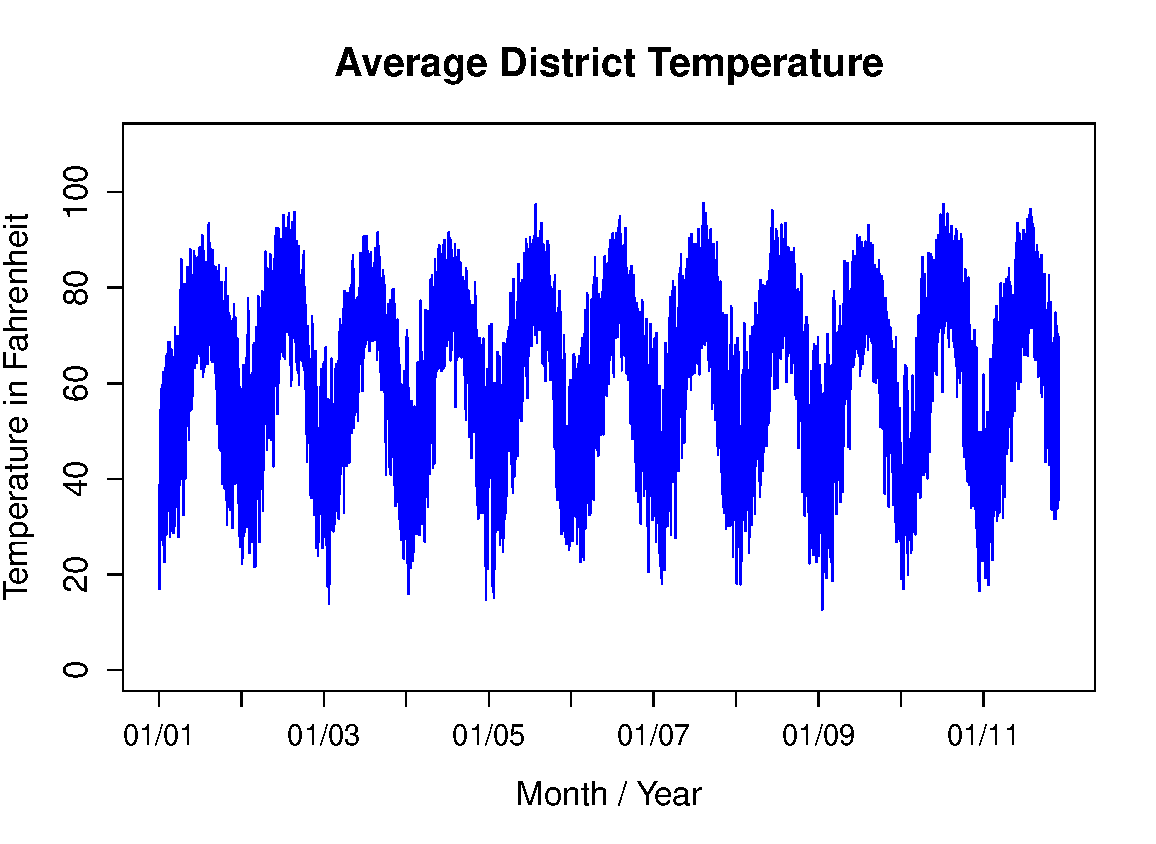
\includegraphics[width=\linewidth]{gfx/avg-district-temp-fahrenheit.pdf}
\label{subfig:avg-temp-fahrenheit}
\end{subfigure}
\begin{subfigure}[b]{.8\linewidth}
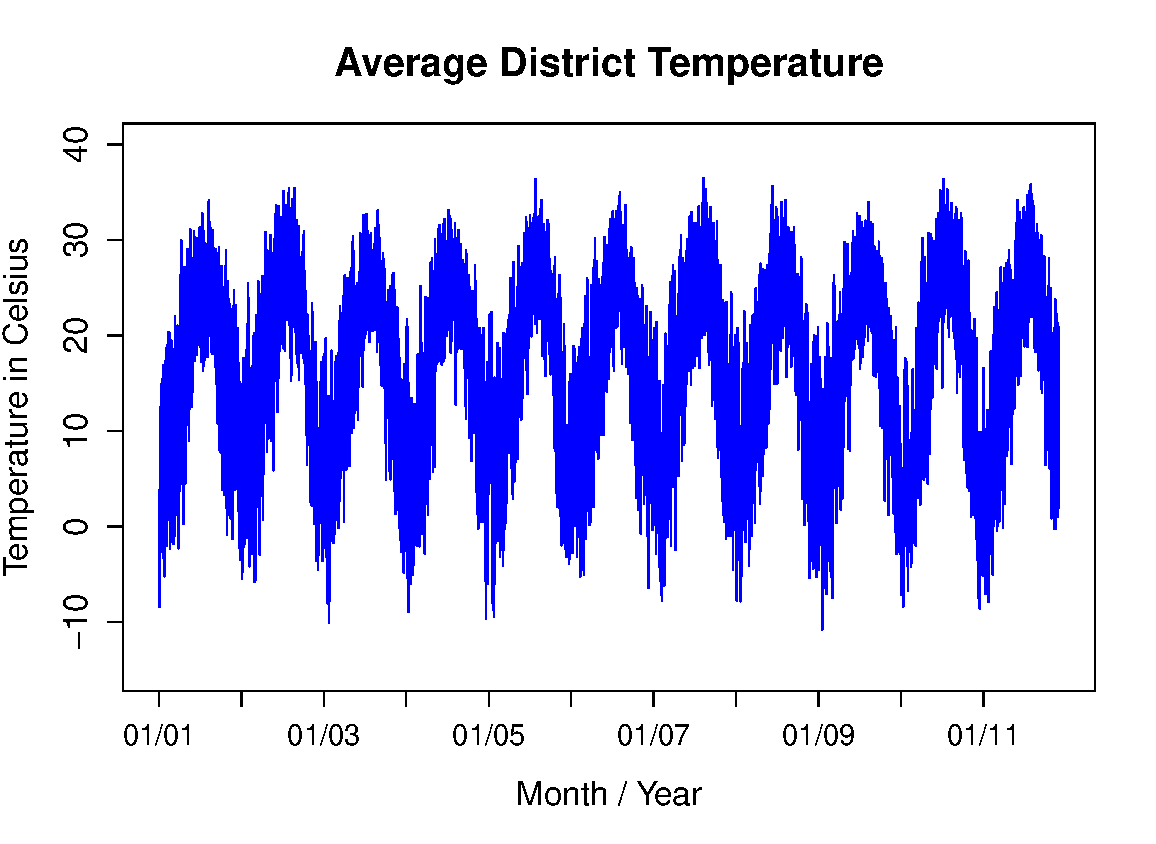
\includegraphics[width=\linewidth]{gfx/avg-district-temp-celsius.pdf}
\label{subfig:avg-temp-celsius}
\end{subfigure}
\caption{Average district temperature over the whole given time period}
\label{fig:temp-lags}
\end{figure}

\begin{figure}[!ht]
\centering
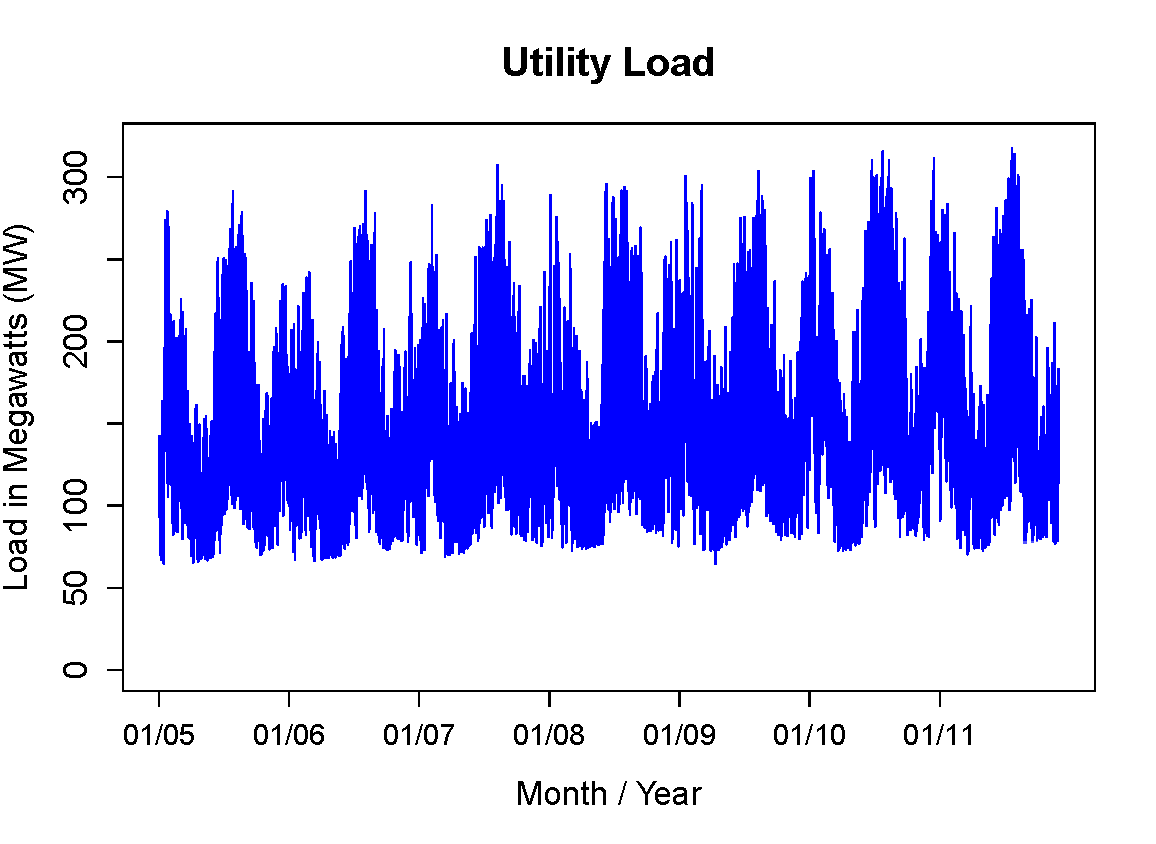
\includegraphics[width=\linewidth]{gfx/utility-load.pdf}
\caption{Utility load of the whole given time period}
\label{fig:utility-load}
\end{figure}

\subsection{Data Cleaning}
An annoying feature of the dataset is that the timestamps are not saved in the international ISO 8601 standard, but as ``MMddYYYY H:m'' without leading zeros for both days and months. Fortunately, the dataset was provided continuously without gaps and therefore the problem could be easily solved by hard-coding the first and last datetimes and using these to generate the needed sequence of datetimes.
%found a way to automatically solve the problem through the linkedin group and a question a participant asked on stackoverflow (http://stackoverflow.com/questions/25386730/parsing-ambiguous-timestamps). 
%However, had to make slight modifications to make it work
%Still didn't work 100%, lost one week on this

\subsection{Temperature Preprocessing}
\label{sec:temp-proc}
%$Corr_X(m) = \frac{\mathbb{E}\[X_t-\mu_x)(X_{t+m})\]}{\var_X}$
We use the hourly average temperature of all weather stations as the basis series for our temperature forecasts (Figure \ref{subfig:avg-temp-2012}).
In other words, we use the average district temperature to predict the district utility load.\par
In another approach we compute the cross-correlations for the 25 weather station (Figure \ref{fig:temp-stations-cc}). The high correlations suggest that, taking into account the inevitable inaccuracy of the temperature forecasts, station 1 can be used for forecasting.\par
%\cite{Fan2010} temperature highly correlated $\rightarrow$ use average
%however, did not use temperature differences: would have led to 25x25 more features

\begin{figure}[ht!]
\centering
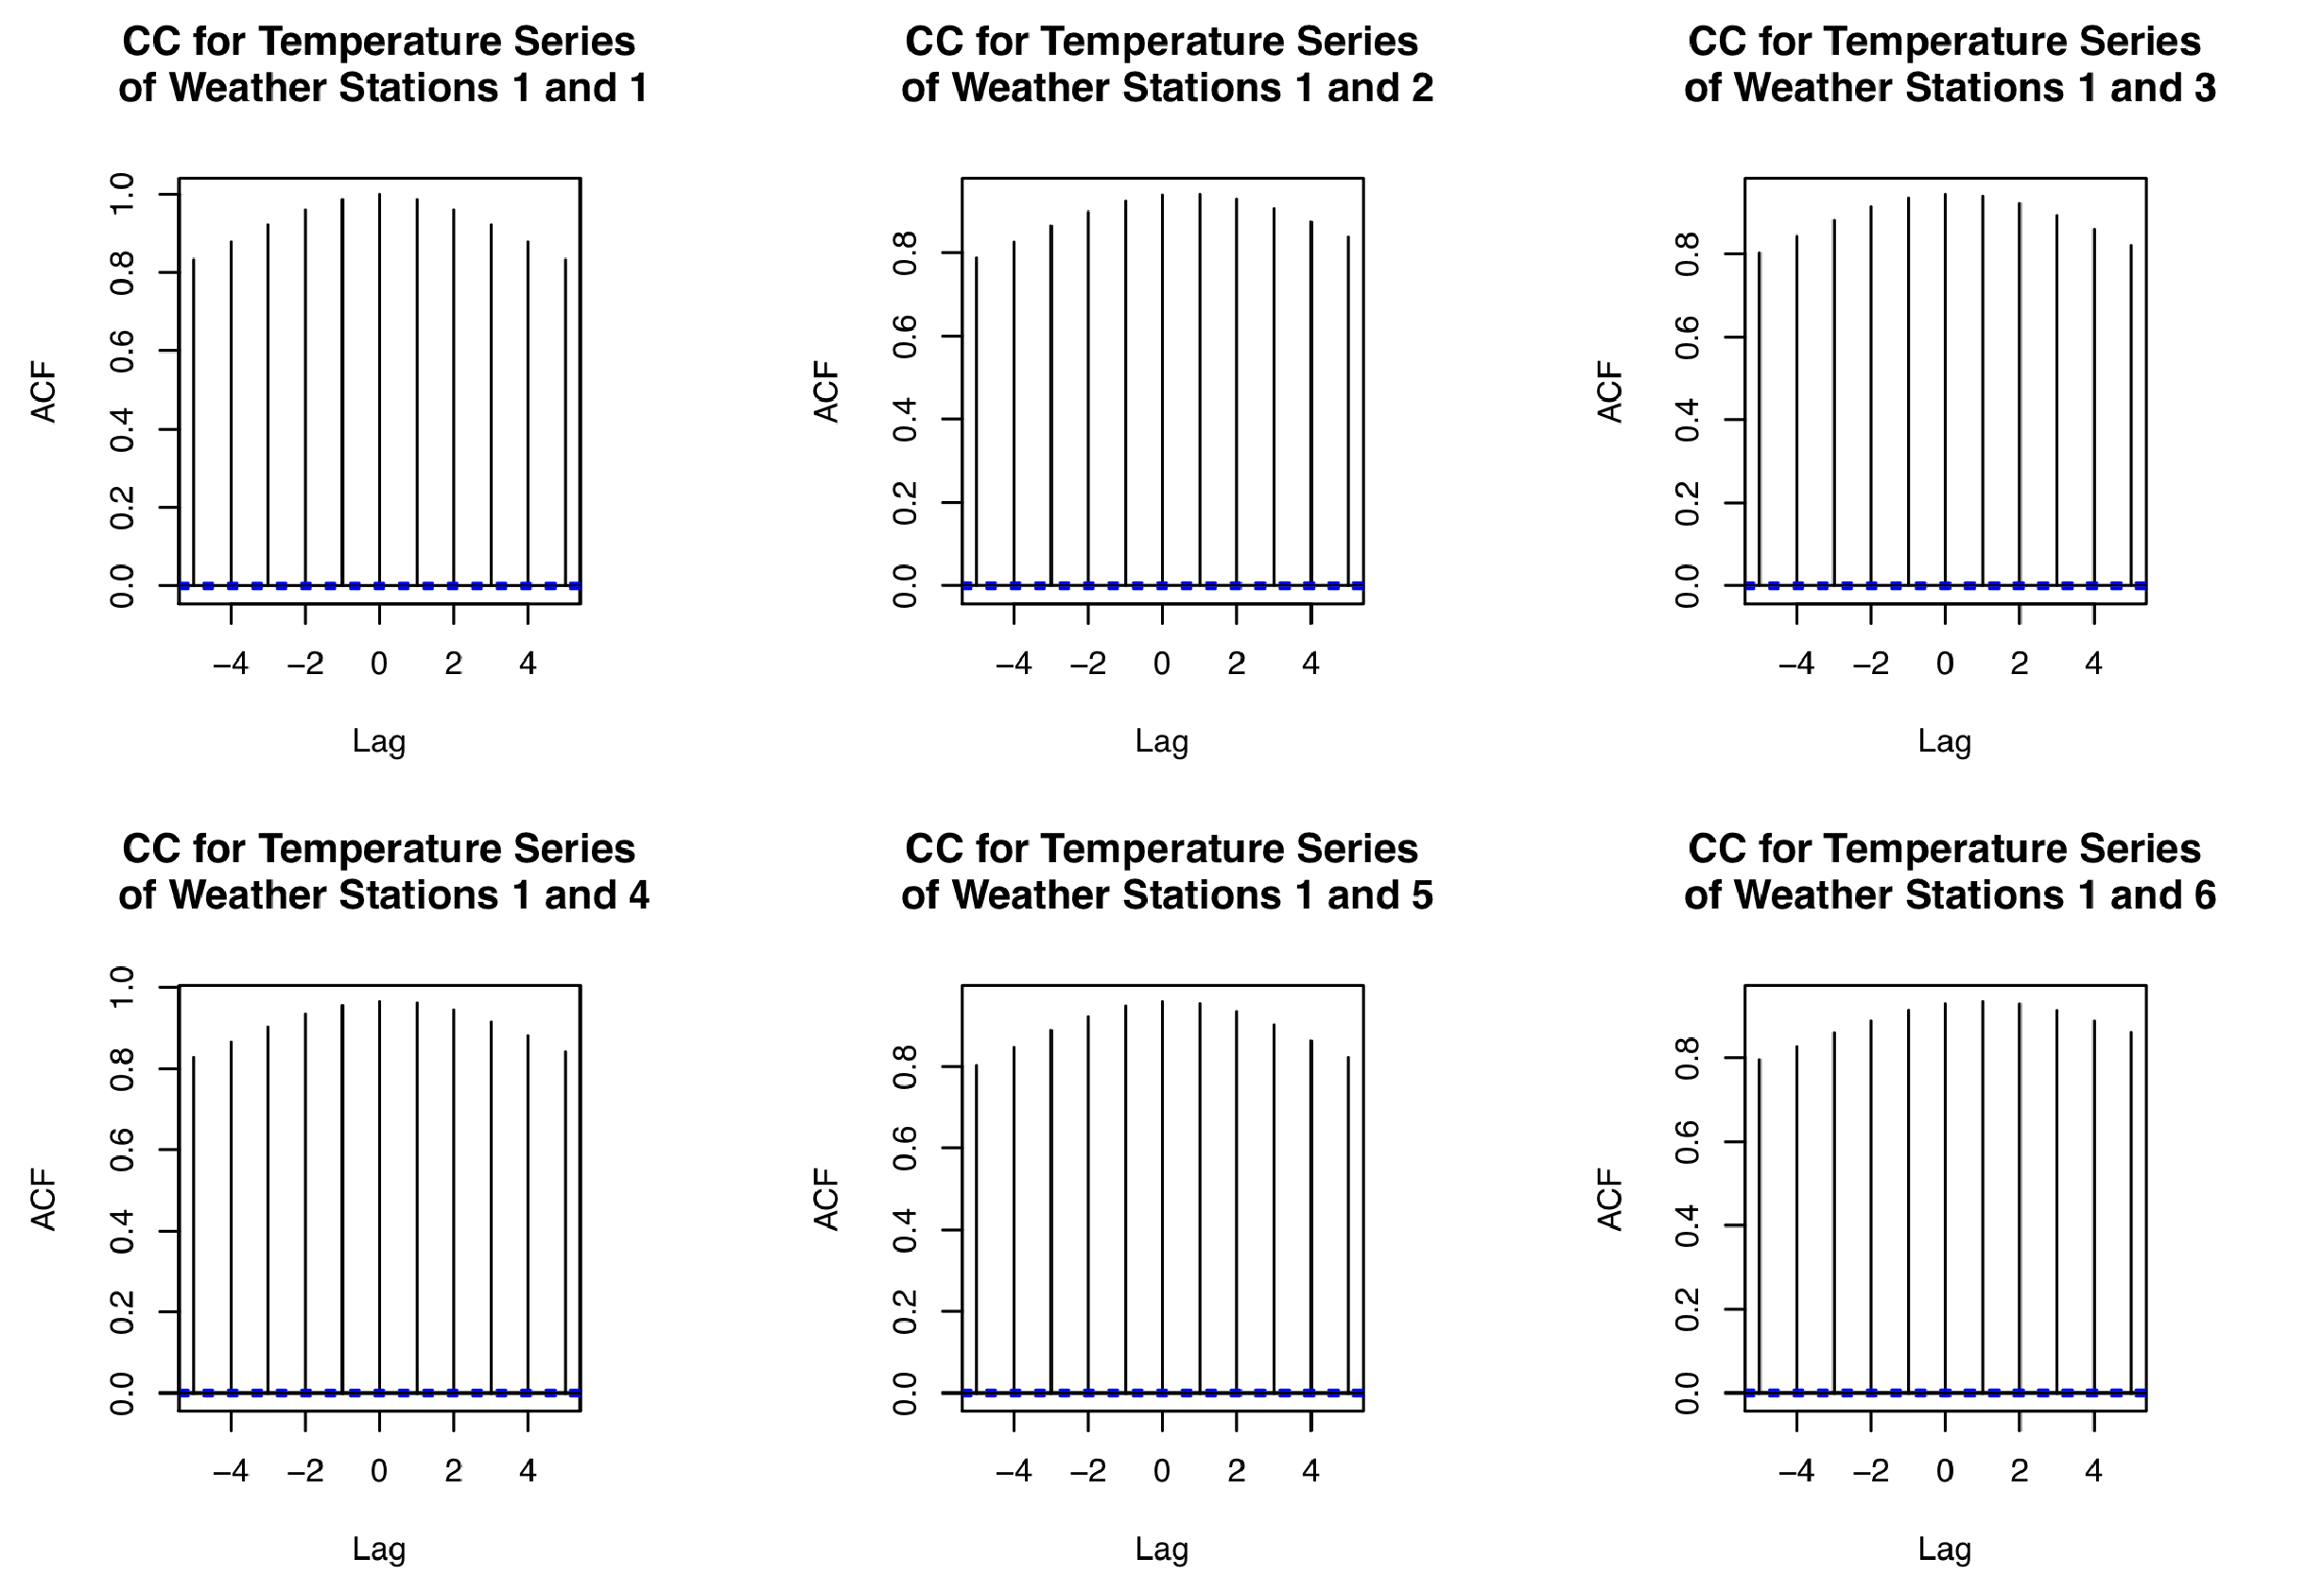
\includegraphics[width=\linewidth]{gfx/weather-station-cc-plots_series1-6_lag5.pdf}
\caption{Cross Correlation Plots of Temperature Station 1 Series with Series of Temperature Stations 1-6. Cross Correlations for Stations 7-25 omitted for convenience of display.}
\label{fig:temp-stations-cc}
\end{figure}
Furthermore we perform a principal component analysis (PCA) on the temperature series and evaluate the use of the first principal component that captures around 90\% of the variance in the temperature (Section \ref{sec:results}).

\begin{figure}[!ht]
\centering
\begin{subfigure}[b]{.8\linewidth}
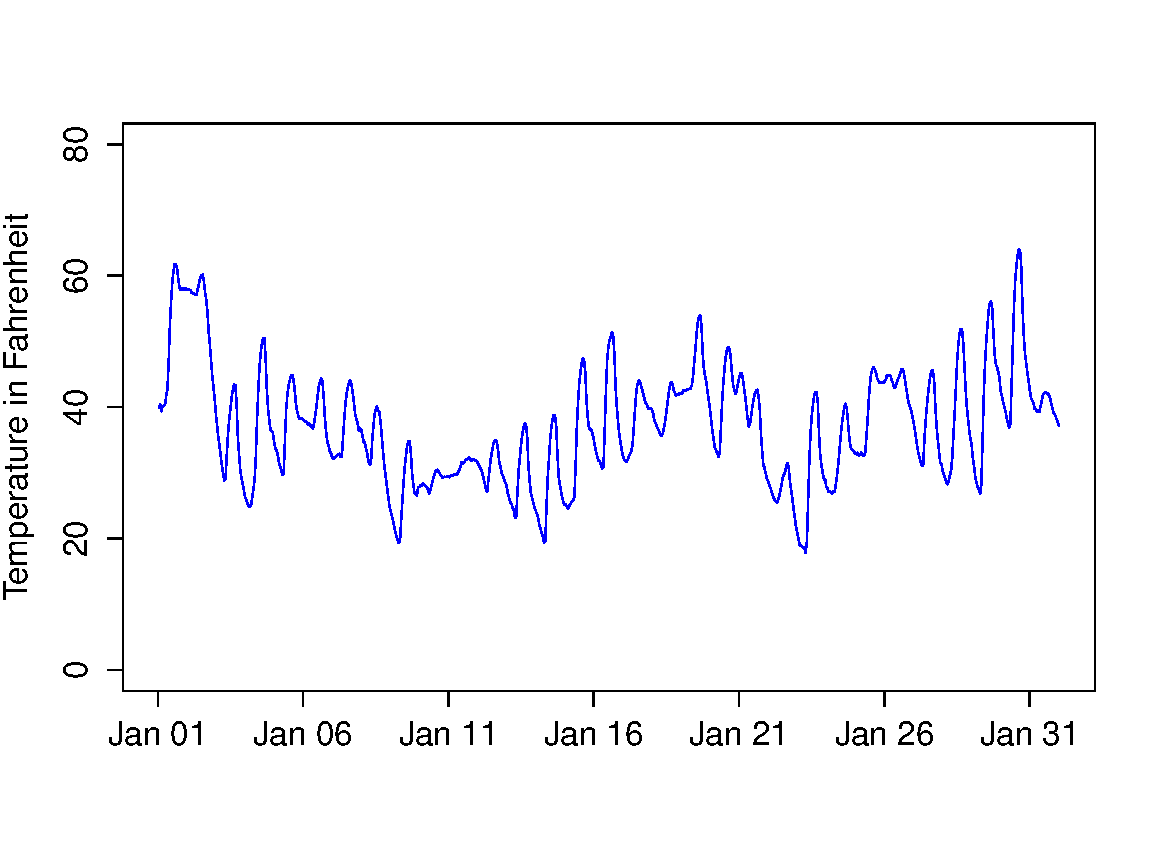
\includegraphics[width=\linewidth]{gfx/avg-temp-2011.pdf}
\caption{Average District Temperature during July 2011}
\label{subfig:avg-temp-2012}
\end{subfigure}
\quad
\begin{subfigure}[b]{.8\linewidth}
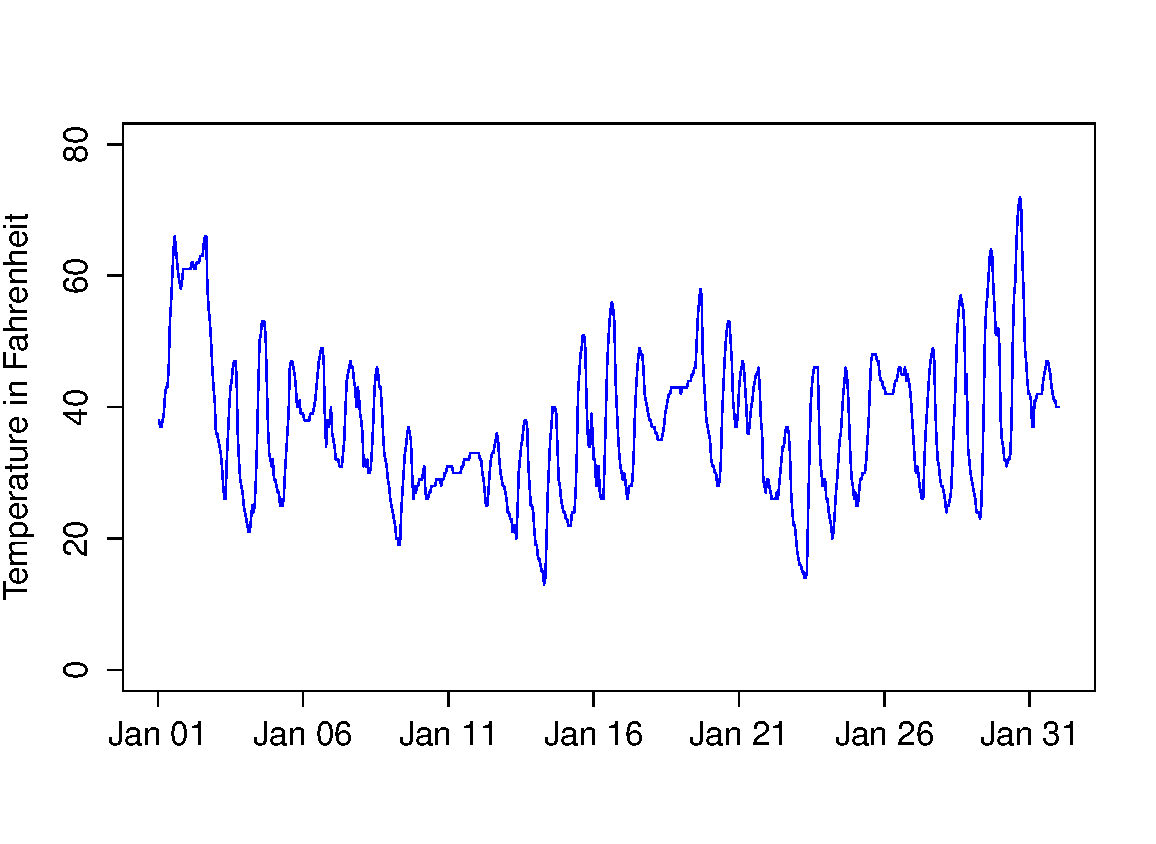
\includegraphics[width=\linewidth]{gfx/temp-station1-2011.pdf}
\caption{Temperature of 1st Weather Station during July 2011}
\label{subfig:temp-station1-2012}
\end{subfigure}
\end{figure}

\subsection{Evaluation Metrics}
The competition requires each of the participants to provide percentile forecasts, that is forecasts of the quantiles $\tau=0.01, 0.02, \dots, 0.99$ with natural lower and upper bounds.
The Evaluation Metric employed to score the contestants' submissionsis the tilted loss/error function also known as the pinball loss/error function. In the following paragraphs let $y$ denote an observation and $\hat{y}$ denote a corresponding forecast while $\xi$ is defined as the residual $y-\hat{y}$.\par
%For a quantile forecast q_a with a/100 as the target quantile, this score L is defined as:
%L(q_a, y) = (1 - a/100) * (q_a - y), if y<q_a;
                %a/100 * (y - q_a), if y>=q_a
%where y is the observation used for verification, a = 1, 2, ..., 99.
\[
  L_{\tau}(\xi)=\begin{cases} \tau \xi & \text{if } \xi \geq 0 \\
                                          (\tau-1)\xi & \text{if } \xi < 0 
                                  \end{cases} \quad\text{where } \xi=(y-\hat{y})
\]
%\tau ist Steigung wenn \xi>=0 und Gefälle wenn \xi<0
To evaluate the full predictive densities, this score is then averaged over all target quantiles, from 0.01 to 0.99, for all time periods throughout the forecast horizon. The lower the pinball score, the better the forecast.

\begin{figure}[ht!]
\centering
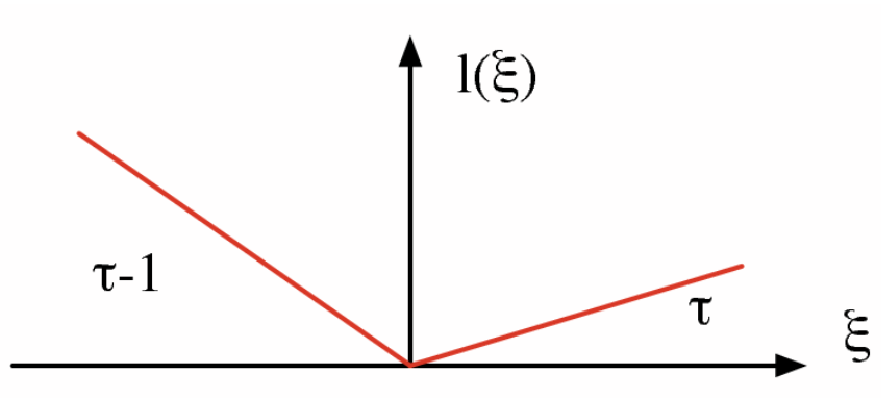
\includegraphics[width=\linewidth]{gfx/pinball.pdf}
\caption{The tilted loss function for 50th, $\tau=0.5$, and 75th, $\tau=0.75$, quantile \cite{Takeuchi2005}.}
\label{fig:pinball}
\end{figure}
In our own evaluation of forecasts, we further use some well-established point error metrics, for the simple reason that we generate our quantile predictions starting from a point prediction. The measures are the Mean Average Error (MAE), Root Mean Squared Error (RMSE) and Mean Absolute Percentage Error (MAPE).\par
The MAE and RMSE measures are the two most common scale-dependent errors, meaning that the residuals $\xi_i$ (for ith observations) are on the same scale as the data. Hence, MAE and RMSE are in units of Fahrenheit or Mega Watt for our data set. 
\[
  \text{MAE}=\mathbb{E}[\xi_i]
\]
\[
  \text{RMSE}=\sqrt{\mathbb{E}[\xi_i]}
\]
As a percentage error the MAPE measure is scale-independent. In our case it is useful for giving an immediate sense of the relative scale of the error.
\[
  \text{MAPE}=\mathbb{E}\left[\left| \frac{100\xi_i}{y_i} \right|\right]
\]
The measure is undefined for $y_i=0$. Fortunately, in our dataset all values are several integers larger than zero for both load and temperature series so that the measure is neither undefined or affected by extreme values.
%source: Rob Hyndman, Forecasting principles and practice, https://www.otexts.org/fpp/2/5


\section{Feature Selection}
In the following paragraphs we explain the methodology we use to obtain our final feature selection for both temperature and load forecasting. The choice of features is limited to calendar features for temperature forecasting, because the only additional data allowed in the competition are Federal US holidays and the forecasting horizon is set to 1 month ahead.
\subsection{Time Lags}
\label{sec:time-lags}
First of all, we want to find out which previous values can be useful in a prediction. Given a time horizon of 1 month we would like to forecast the whole month using only one model for reasons of convenience. This circumstance induces a time lag of minimum 28 days for the month of february. For simplicity of implementation we define the same minimum lag of 31 for every month of the year.   
In order to choose the lag variables we interpret the cross-correlation of observations $y_i$ and $y_{i-k}$, for different hourly lags $k=1,2,..$, of both temperature and load time series in (Figure \ref{fig:temp-lags}).
This serial correlation of observations is known in statistics as autocorrelation and demonstrates the similarity of observations in a series as a function of the time lag between them.
% series are not Second Order Stationary Processes?
%When your data is nonstationary (inhomogeneous), autocorrelation can still be defined and computed, but will now depend on the pivot (=reference) point as well, nut just the distance (=delay, lag) between points. As a result, the autocorrelation becomes a functional, no longer a function. In the discretized (sampled) case, this functional becomes a matrix.
Using the empirical mean and standard deviation of our target series $Y=\{y_1, y_2, \dots, y_i, \dots, y_N\}$ we can compute the autocorrelation for lag k with:
\[
  \mathcal{R}(k)=\frac{\mathbb{E}\left[(y_i-\mu)(y_{i-k}-\mu)\right]}{\sigma^2}
\]

As can be seen in both figure \ref{subfig:avg-temp-7days} and \ref{subfig:temp-station1-7days} the highest autocorrelations occur with a periodicity of 24 hours. Therefore we choose 24 hours as the base number for selecting the time lags of our predictions. The average temperature series in the former figure displays less variance in the correlations than the first station in the latter because the hourly temperature is less extreme due to the averaging over zones. 

\begin{figure}[!ht]
\centering
\begin{subfigure}[b]{.49\linewidth}
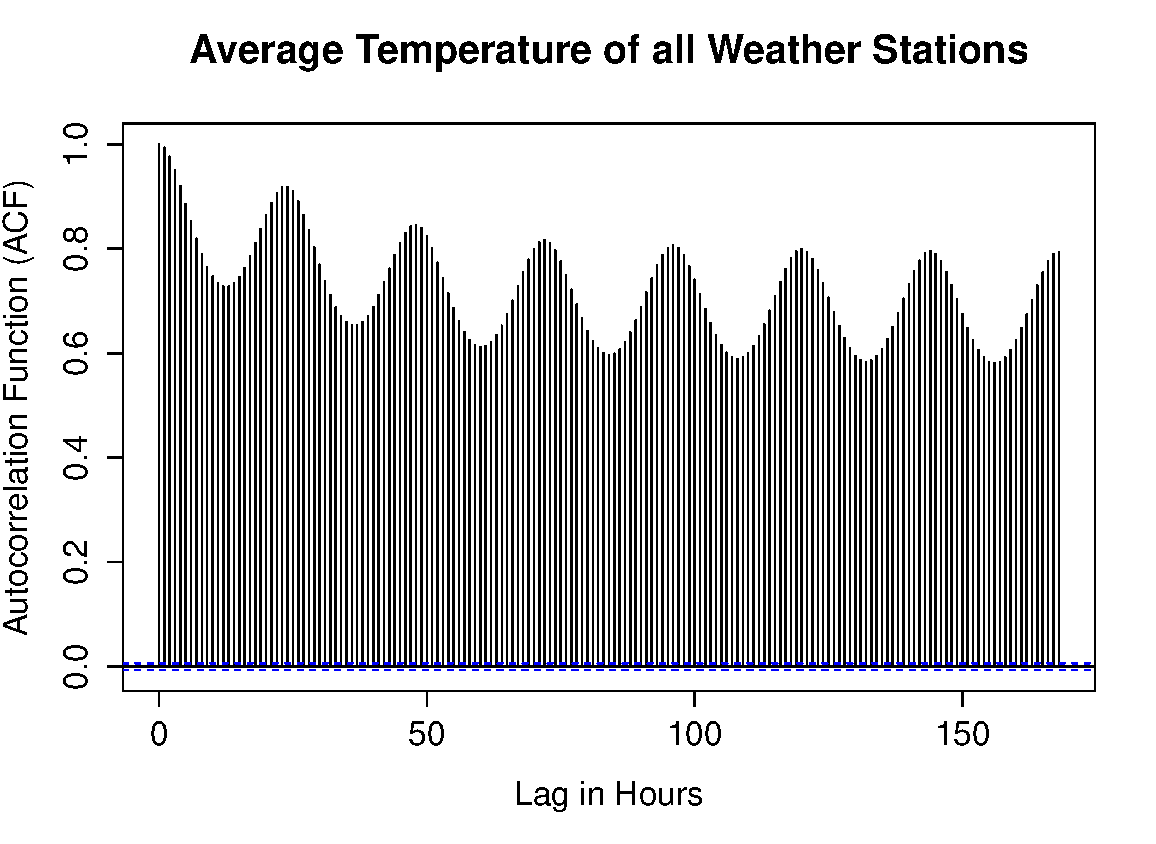
\includegraphics[width=\linewidth]{gfx/acf_avg_temp_7days.pdf}
\caption{time lag: 7 days, 168 hours}
\label{subfig:avg-temp-7days}
\end{subfigure}
\begin{subfigure}[b]{.49\linewidth}
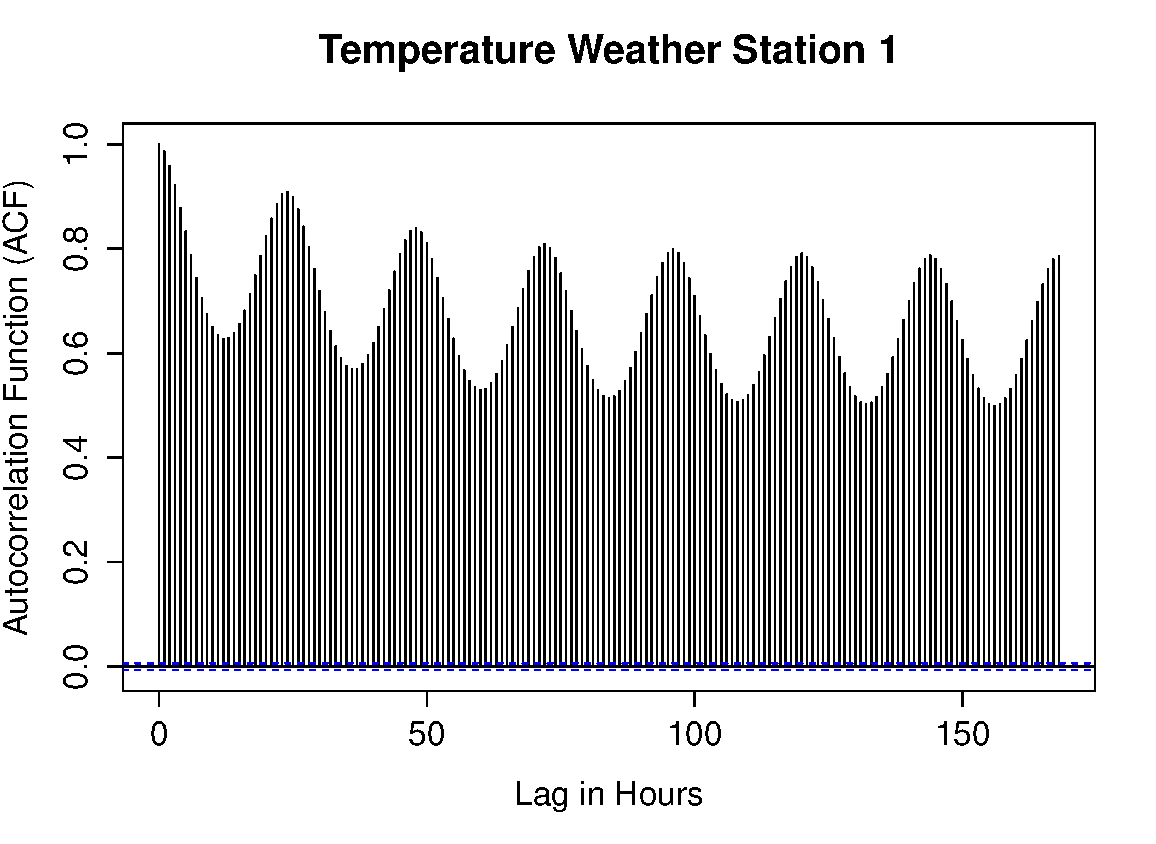
\includegraphics[width=\linewidth]{gfx/acf_temp_station1_7days.pdf}
\caption{time lag: 7 days, 168 hours}
\label{subfig:temp-station1-7days}
\end{subfigure}
\caption{Autocorrelation function estimates for hourly average temperature of district and hourly temperature at station 1 for different maximum time lags.}
\label{fig:temp-lags}
\end{figure}

Figure \ref{fig:acf-load} shows the autocorrelation function of the load series for different maximum lags. As can be seen the load correlations also have a periodicity of 24 hours (Figure \ref{subfig:acf-load-7days}). The other figure \ref{subfig:acf-load-35days} show that after an initial exponential decrease the correlations decrease near linearly. Since the type of day has an influence on the utility load (Section \ref{sec:calendar}), we set the basis for time lags to $7\cdot24$ hours for the load and the minimum time lag for monthly load forecasts therefore to 35 days.

\begin{figure}[!ht]
\centering
\begin{subfigure}[b]{.49\linewidth}
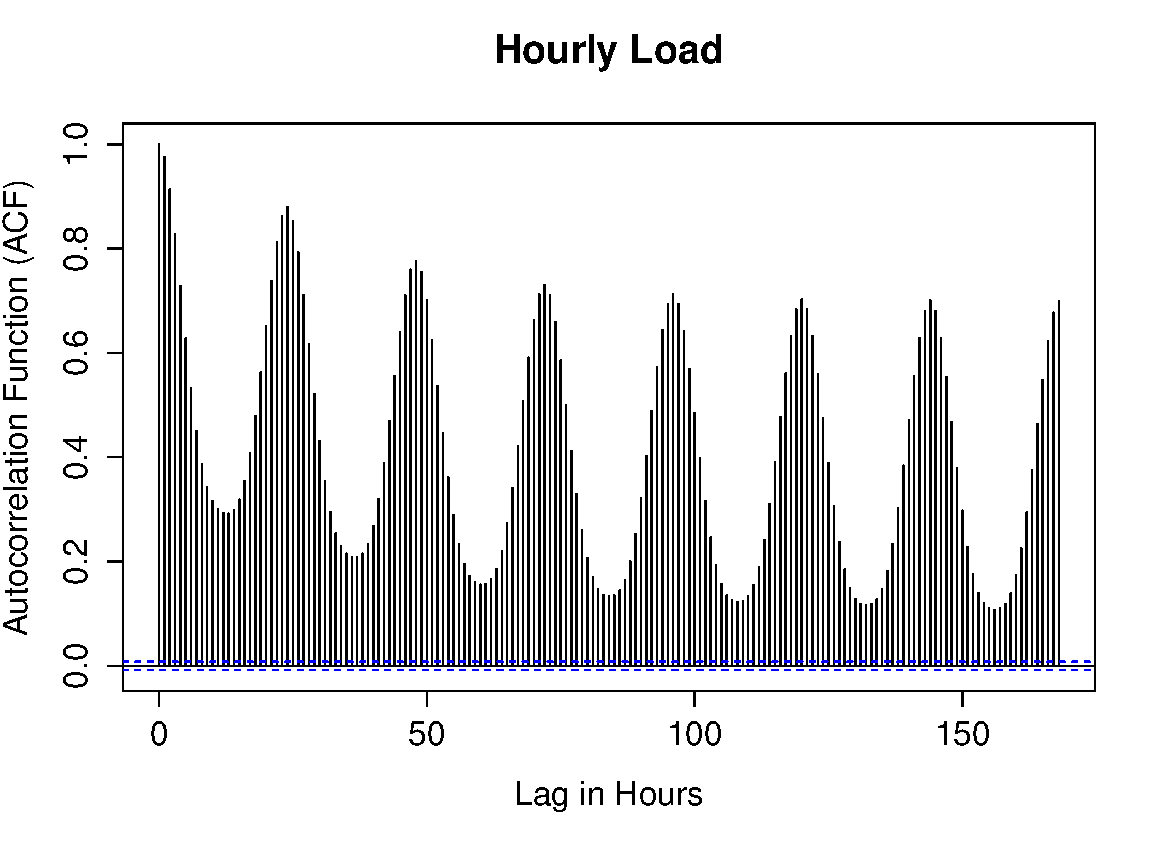
\includegraphics[width=\linewidth]{gfx/acf-load-7days.pdf}
\caption{time lag: 7 days, 168 hours}
\label{subfig:acf-load-7days}
\end{subfigure}
\begin{subfigure}[b]{.49\linewidth}
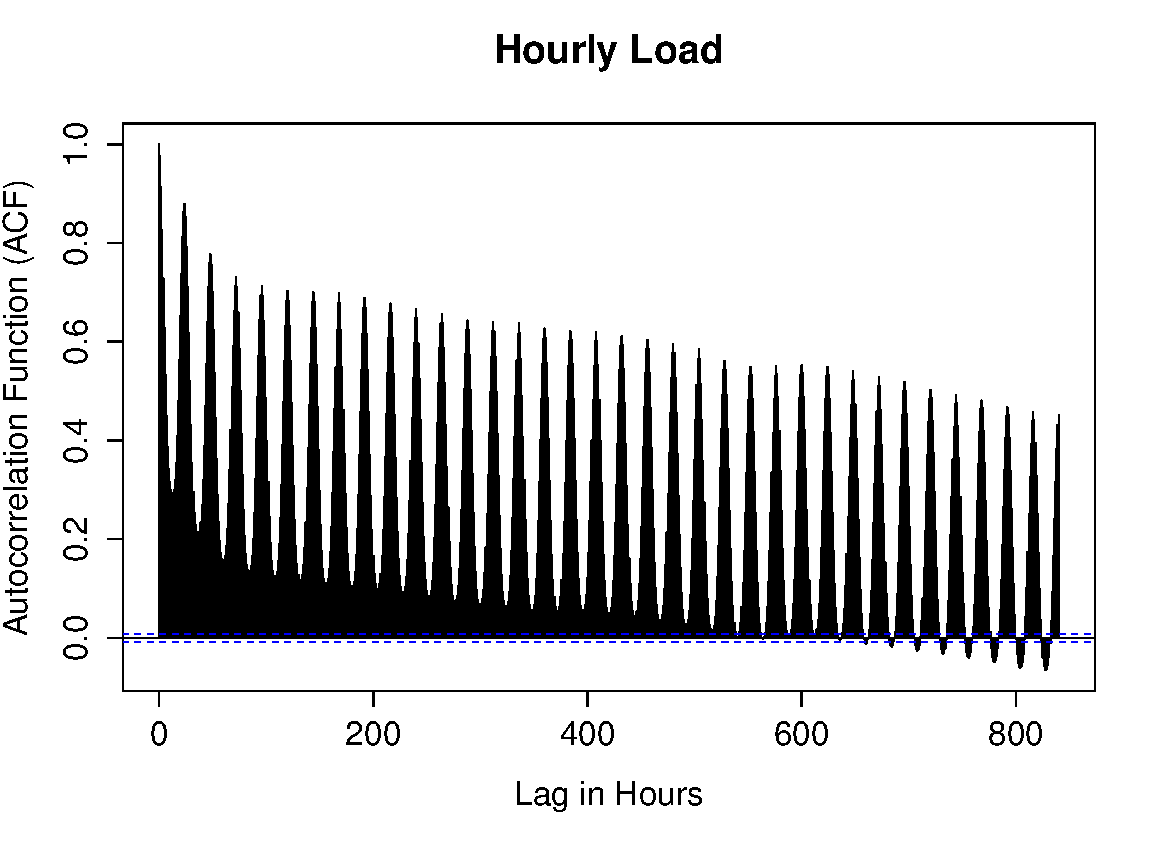
\includegraphics[width=\linewidth]{gfx/acf-load-35days.pdf}
\caption{time lag: 35 days, 840 hours}
\label{subfig:acf-load-35days}
\end{subfigure}
\caption{Autocorrelation Function Estimates for hourly load data in MW for different maximum time lags.}
\label{fig:acf-load}
\end{figure}

\subsection{Calendar Features}
\label{sec:calendar}
Figures \ref{fig:temp-lags} and \ref{fig:acf-load} have shown both temperature and load series to possess daily frequency. We therefore extract the hour of the day from the datetimes and use it as a feature.\par
Figure \ref{fig:seasonality} demonstrates the seasonal change of temperature and load throughout the year. In order to capture the seasonality in our models for both temperature and load, we use the time of the year as a feature. We indicate the progress of the current year with a continously growing sequence
\[
\text{toy}=\{\text{toy}_1, \text{toy}_2, \dots, \text{toy}_i, \dots\},\quad \text{toy}_i \in [0,1] 
\]
where the endpoints 0 and 1 only approximately, due to leap years, correspond to January 1st 1am and and subsequent midnight January 1st (Section II.B \cite{Goude2014}). An alternative is to use a categorical variable indicating the present month.

\begin{figure}[!ht]
\centering
\begin{subfigure}[b]{.49\linewidth}
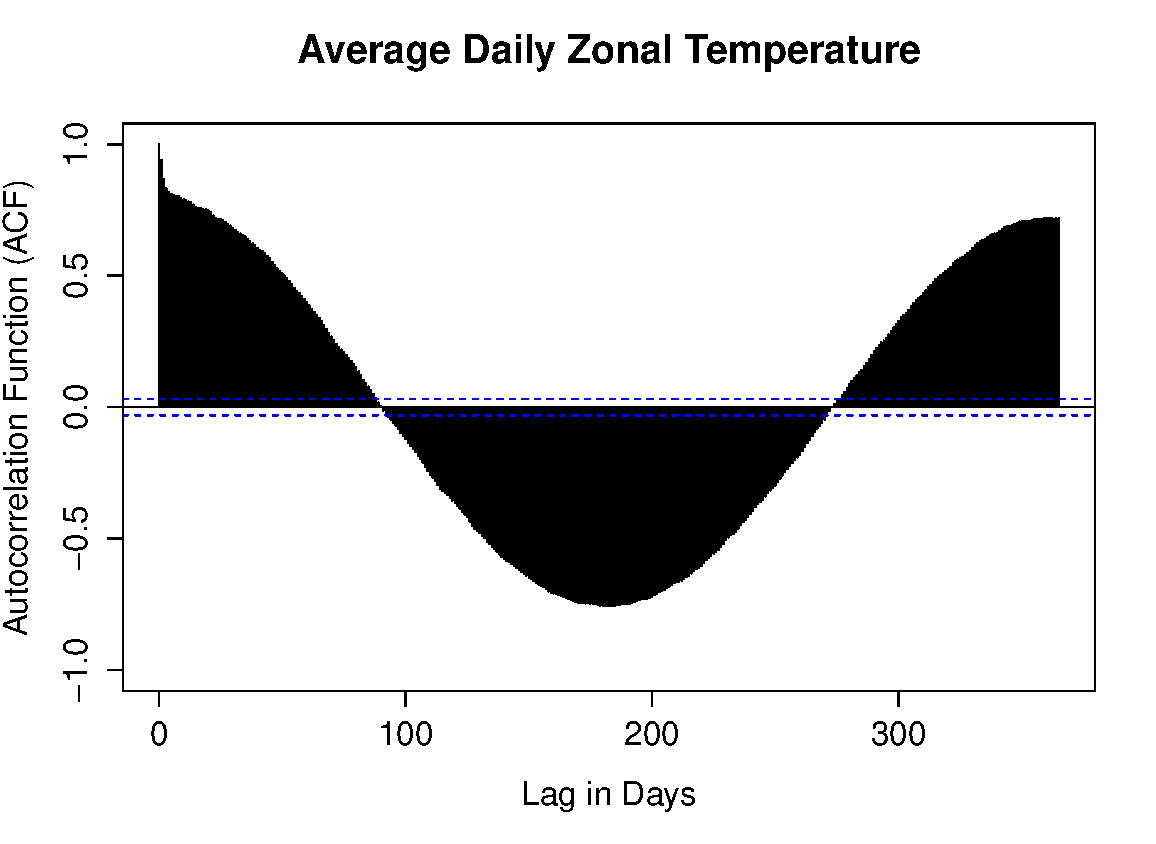
\includegraphics[width=\linewidth]{gfx/daily-avg-temp-1year.pdf}
\label{subfig:acf-temp-1year}
\end{subfigure}
\begin{subfigure}[b]{.49\linewidth}
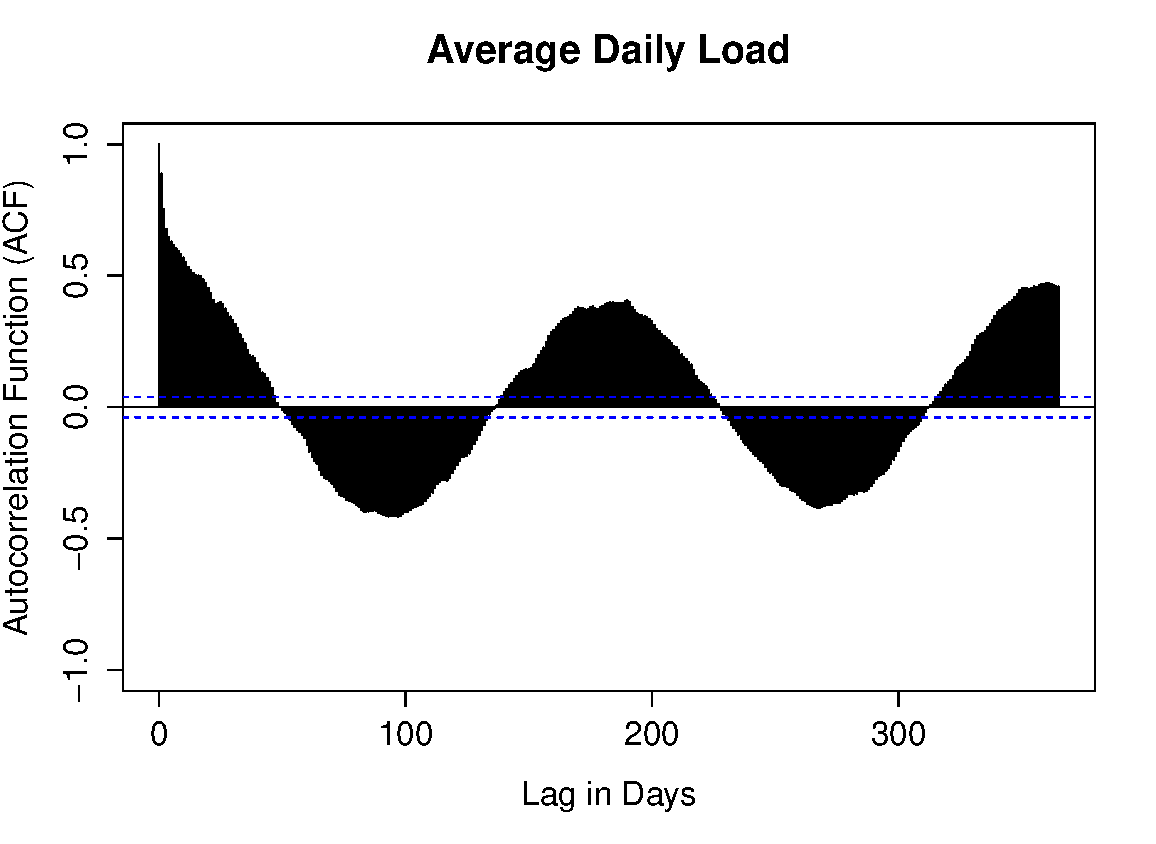
\includegraphics[width=\linewidth]{gfx/avg-daily-load-1year.pdf}
\label{subfig:acf-load-1year}
\end{subfigure}
\caption{Autocorrelation function estimates for daily averages of both hourly average temperature for the district and the load for a maximum lag of 1 year.}
\label{fig:seasonality}
\end{figure}
The features we discussed so far are analyzed for both temperature and load forecasting later in this report (Section \ref{sec:results}). The nature of the load data allows us to proceed with the extraction of another feature, the day of the week as introduced by \cite{Hong2010}. Energy consumption does not only depend on the climatic circumstances, but also directly on the calendar events, because consumption patterns vary between the different days of the week, weekends and holidays due to human activity (Section 2.6 \cite{HongThesis}). 
%The energy utility data does not show clear patterns when probing \ref{fig:coming}. 
As proposed in \cite{Hyndman2010} section IV.A, we use different approaches of marking the days of the week, numbering the days of the week from 1 (Sunday) to 7 (Saturday) and assigning weekdays and weekend days with 1 and 2 respectively.\par
The only external data source allowed for the GEFCom load forecasting track are \href{http://archive.opm.gov/Operating\_Status\_Schedules/fedhol/2014.asp}{U.S. federal holidays} for the time span of the provided data. This gives us the possibility to additionally detect holidays and assign them another integer (8) in the approach of consecutively numbering the days of the week.\par

\begin{table}[h]
\centering
\begin{tabular}{@{}llllllllll@{}}
\toprule
 Type & Mon & Tue & Wed & Thu & Fri & Sat & Sun & Holiday \\ \midrule
SDAYT & 2 & 2 & 2 & 2 & 2 & 1 & 1 & - \\
WDAYT & 2 & 3 & 4 & 5 & 6 & 7 & 1 & - \\
DAYT & 2 & 3 & 4 & 5 & 6 & 7 & 1 & 8 \\ \bottomrule
\end{tabular}
\caption{Different assignments of integers for days of the week. SDAYT stands for simple day type (weekdays vs. weekends), WDAYT for week day type numbering all days of the week and DAYT includes holidays.}
\label{my-label}
\end{table}

\section{Forecasting Methods \& Methodology}
In this section we briefly review the forecasting models used during this project. On the one hand we use a generalization of the Linear Model (LM), the generalized additive model (GAM), and on the other basic implementations of established machine learning methods such as neural networks (NN) and random forests (RF). For reasons of priority, we did not use our own implementations, but rather those that have been made available through R packages. With every method we create several models using different subsets of features for evaluation of both temperature and load forecasting (Section \ref{sec:results}).

\subsection{Linear Model (LM)}
%instead of linear predictor refer to univariate response variable
We use the ordinary least squares (OLS) linear regression model as a benchmark method to interprete the prediction power of the other methods. OLS assumes the residuals to follow a normal distribution $\epsilon \sim \mathcal{N}(\mu, \sigma^2)$. The linear predictor is therefore the sum of a linear combination of covariates and Gaussian noise and the predictor $y = \vec{\phi}^T \vec{x} + \epsilon$. The vector of covariates $\vec{x}$ contains the pre-selected features, i.e. the temperature variable and the calendar effects, as well as the bias term $x_0$ and $\vec{\phi}$ represents the vector of coefficients that are to be learnt with least squares approximation.

\subsection{Generalized Additive Model (GAM)}
The standard linear regression model we use is a generalized linear model with a gaussian distribution and an identity link function. For the general additive model we employ \cite{Wood2006} we will not change the link function, since we are going to use a Gaussian distribution here as well. However, generalized additive models allow a generalization on top of that of the incorporation of other distributions as in Generalized Linear Models, that of \emph{nonlinear predictors}. Hence, assuming a Gaussian error model the linear predictor turns into a nonlinear predictor with a combination of smooth functions of the predictor variables: $y=s_1(x_1)+s_2(x_2)+\dots+s_p(x_p)+\epsilon$, where the $s(x_i)$ are smooth functions of the chosen features. Note that not all covariates need to be wrapped in smooth functions.\par
Since the nonlinear functions are smooth they can be estimated by penalized regression in a spline basis \cite{Nedellec2014}, \cite{GAMS}:
\[
  s_i(x)=\sum_{j=1}^{k_i}\beta_{i,j}\varphi_j^i(x)
\]
Here $k_i$ is the dimension of the spline basis and $\varphi_j^q$ are the corresponding spline functions. The default splines for GAMs in the \textbf{mgcv} package are thin-plate splines \cite{Wood2003} where $\varphi(x)$ is of the family of radial basis functions. The focus of this project was on forecasting workflow and feature selection, so that different spline specifications have not been tried out.\par
%Show model output and how degrees of freedom are chosen?

\subsection{Neural Network (NN)}
Neural networks are powerful machine learning algorithms. They exist in many varieties, with feedforward neural networks being the most basic. In our predictions we use a simple feedforward neural network with one hidden layer with a varying number of hidden units (from now on referred to as \textbf{hunits}) and a linear output unit. Such a network can be easily used for regression using the R package \emph{nnet} \cite{Venables2002}.

\subsection{Random Forest (RF)}
Random forests \cite{BreimanRF} are a powerful ensemble method for capturing nonlinear dependencies that does not require significant tuning. They employ decision trees which are very popular in machine learning. To avoid the effects of overfitting a bunch of random decision trees are automatically. ``Each simple tree gives its prediction, and these are then aggregated using the mean of the individual predictions. Each tree model assigns a class to the new vector of covariates, based on the recursive partitioning. Then, the prediction is the mean value of the responses that correspond to this class.'' \cite{Nedellec2014}. A decision tree can process continuous and discrete covariates, as is the case with our features, while providing a continuous response. Chapter 15 of \cite{hastie01statisticallearning} provides the reader with a detailed introduction to the subject. For simplicity, we use the \emph{randomForest} R package \cite{Liaw2002} and try the algorithm for a varying number of trees. We will refer to this variable in the following as \textbf{ntrees}.

%case where the response is continuous and the covariates are both continuous and discrete.
%data \{yi,x1,i,...,xp,i; i = 1,...,n\}. In this short presentation, we focus on the
%The estimation is done by averaging many simple tree models. Each of the tree models is a recursive partitioning of the space of covariates, in order to obtain classes of observations that maximize some purity criterion for the response (e.g., reduce the intra-class variance). 
%If the tree models are built to be de-correlated, the averaging step will reduce the variance of the random forest estimator significantly. In order to build a de-correlated tree model, the random forest adds two layers of controlled randomness to the data. The first layer is generated by a bootstrap sampling of the observations, while the second one is produced from a random draw from a subset of covariates on each partitioning step.
%For a new vector of covariates (x1,n+1 , . . . , xp,n+1 ), we can predict the value of the non-observed response yn+1 using the estimation fˆ of f , obtained using n data points. To do this, each simple tree gives its prediction, and these are then aggregated using the mean of the individual predictions. Each tree model assigns a class to the new vector of covariates, based on the recursive partitioning. Then, the prediction is the mean value of the responses that correspond to this class.

\subsection{Time series cross-validation}
After creating the features for the whole dataset, we run through the whole dataset, temperature and load respectively, in a rolling fashion to create our predictions. This approach can be described as ``forecast evaluation with a rolling origin''. However, since, according to Hyndman \cite{Rob}, it is the natural and obvious analogue to leave-one-out cross-validation for cross-sectional data origins, we can call it ``time series cross-validation''.\par
Forecasts are created with two time horizons: 1 month and 1 week. The idea behind the weekly forecasts is to allow for shorter, but increasing time lags in week 1, 2, 3 and 4 of the month constituting the time horizon. The forecasts of week 1 to 4 are then combined with the rest of the forecast from the monthly forecasts.

\subsection{Creation of Quantiles}
We use the residuals $\xi=y-\hat{y}_i$ created during training to create the desired percentile forecast by offsetting the mean of the estimated gaussian distribution of residuals with the point forecasts produced by the mentioned methods and models.
%Error shoud ideally have zero mean

%\subsection{Monthly vs. weekly forecasting}
%\subsection{Monthly vs. weekly training}

\section{Results}
\label{sec:results}
In this section we discuss the score of several configurations of the methods mentioned above with respect to the leaderboard of GEFCom 2014. We do this for different feature combinations. First, temperature forecasts are addressed and then load forecasting with and without temperature.

\subsection{Temperature}
In this section we display the results for temperature forecasting. Figure \ref{fig:temp-results} is comparison of the best performing method configurations for monthly and weekly forecasting horizons. Over validation period the feedforward neural network with 30 hidden units (hu) has the best performance on average with two different models: with and without the use of a recent lag variable from before the forecasting horizon. The monthly and weekly MAPE score are 12.04\% and 12.17\% respectively. Significant difference 
% DLAG by season
\begin{figure}[!ht]
\centering
\begin{subfigure}[b]{\linewidth}
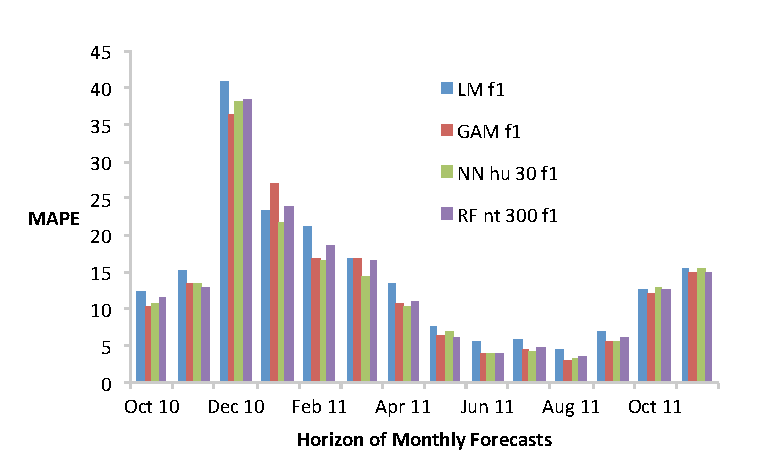
\includegraphics[width=\linewidth]{gfx/results/temp/TEMP-MONTHLY-BEST-COLUMNS.pdf}
\caption{Forecasting 1 month ahead}
\label{subfig:best-temp-methods-monthly-pred}
\end{subfigure}
\begin{subfigure}[b]{\linewidth}
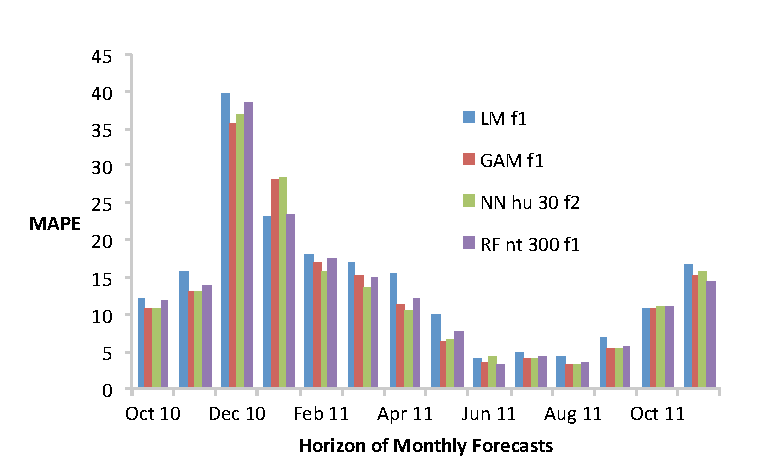
\includegraphics[width=\linewidth]{gfx/results/temp/TEMP-WEEKLY-BEST-COLUMNS.pdf}
\caption{Forecasting 1 week ahead 4 times}
\label{subfig:best-temp-methods}
\end{subfigure}
\caption{MAPE scores for the best performing temperature method configurations. ``f1'' stands for ``formula 1'' which contains the most recent possible time lag variable, a time lag variable of 365 days, the time of year and the hour of the day. The feedforward neural network formula in subfigure \ref{subfig:best-temp-methods} excludes the recent time lag variable.}
\label{fig:temp-results}
\end{figure}
A simpler way of trying to predict the temperature is to use the mean of the sequence of $k\cdot 365 \text{ days}, k=1,2,\dots$ time lags applied to the temperature. However, the resulting score of 22.04\% over the entire forecasting horizon is simply too high and not competitive with the method configurations shown in Figure \ref{fig:temp-results}. 

\begin{comment}
\subsubsection{Effect of the time horizon}
Using the prediction horizon of a week allowing for smaller time lags to preceeding values in the series has a positive effect on the prediction of the temperature. In all methods except for the neural network we see improvements from the monthly prediction to the weekly one.
\begin{figure}[!ht]
\centering
\begin{subfigure}[b]{.49\linewidth}
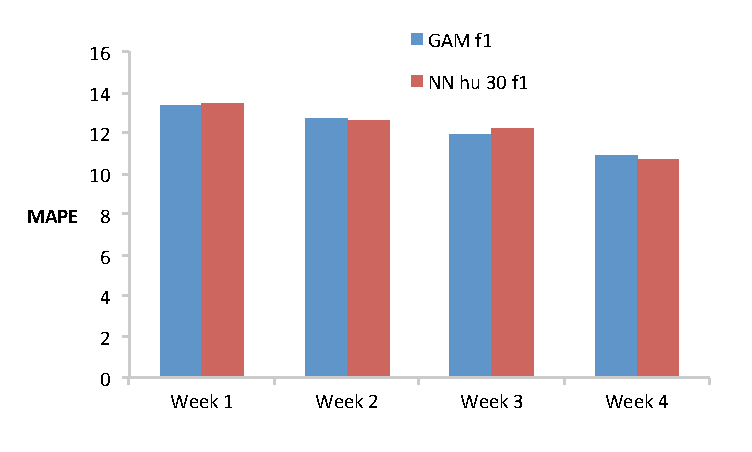
\includegraphics[width=\linewidth]{gfx/results/temp/MAPE-BY-WEEK-DLAG.pdf}
\label{subfig:acf-temp-1year}
\end{subfigure}
\begin{subfigure}[b]{.49\linewidth}
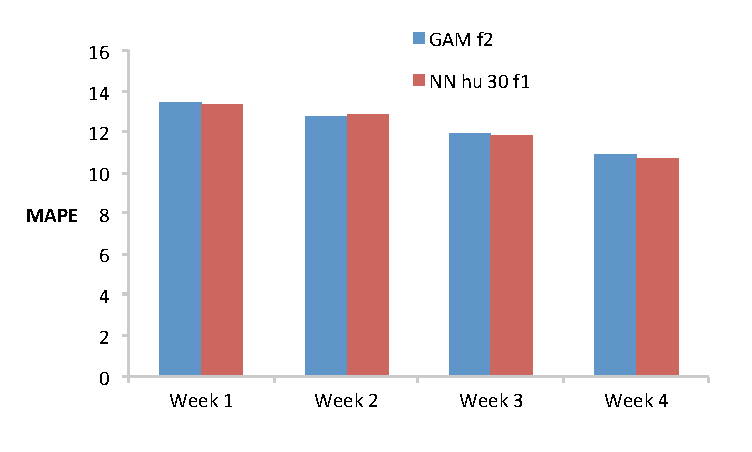
\includegraphics[width=\linewidth]{gfx/results/temp/MAPE-BY-WEEK-NO-DLAG.pdf}
\label{subfig:acf-load-1year}
\end{subfigure}
\caption{MAPE and PINBALL scores for different temp models.}
\label{fig:temp-results}
\end{figure}
%\sout{decide over effect of DLAG $\rightarrow$ effect on temp models} positive effect on weekly prediction
\end{comment}

\subsection{Load Modeling}
The focus of this project is on load forecasting, therefore more effort is made to explain the results for load forecasting. We are more interested in the temperature modeling affects the forecasts than how the temperature modeling itself can be significantly improved. In this section we show results for configurations of GAM, random forest and LM. LM serves the purpose of showing obvious effects of the temperature on the load forecasts, since its forecasts are very fast to simulate. Feedforward neural network load  models are not discussed, because they did not perform well on the load compared to the other methods. Moreover, the forecasting tasks took a long time to run. 

\subsubsection{Effect of Temperature}
To evaluate the effect of the temperature forecasts on the load prediction, we run our models with and without the temperature as a feature. Figure \ref{fig:load-no-temperature} shows the comparison of the MAPE of two different GAM models. Model ``GAM f2'' which does not include the average district temperature as a feature performs significantly worse. Over the whole cross-validation period it scores an average MAPE of 19.18 (1 month forecasting horizon), 18.25 (1 week forecasting horizon), compared to 16.33 and 15.83 respectively for the other model already shown in ``GAM f1''. Additionally to the features used for temperature modeling, these models now include the daytype as a categorical variable and the current, predicted temperature.
\begin{figure}[!ht]
\centering
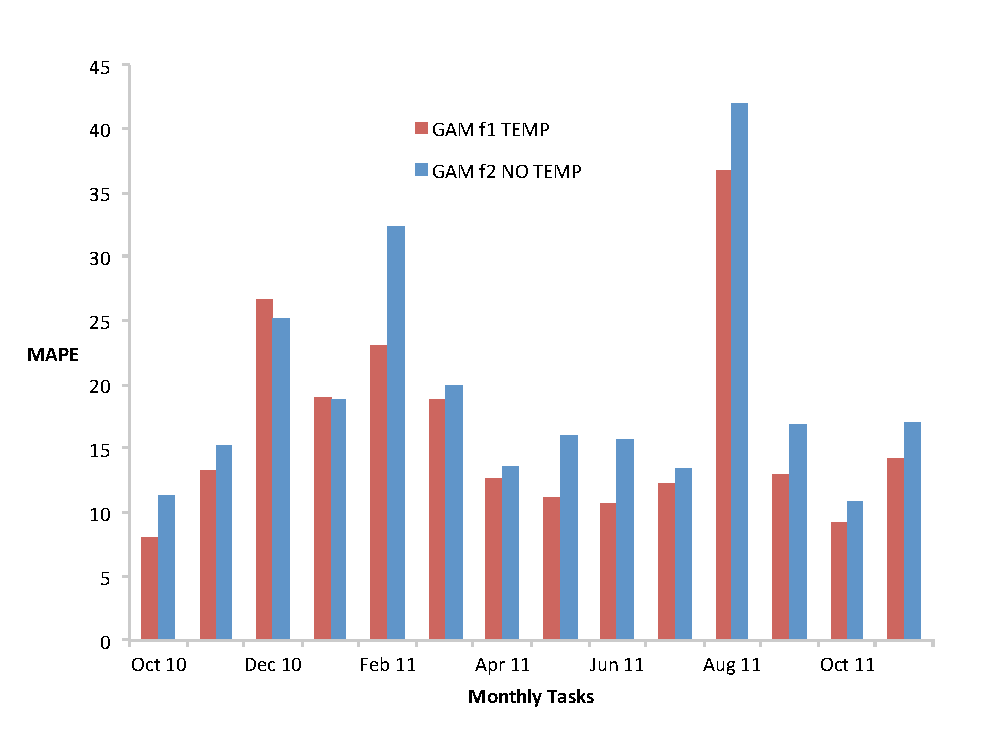
\includegraphics[width=\linewidth]{gfx/results/temp/GAM-temp-vs-no-temp-column.pdf}
\label{subfig:GAM-temp-no-temp}
\caption{MAPE score for models with and without temperature variable. The GAM model without the temperature feature, but otherwise identical, has a significantly higher MAPE. This shows that although the unsophisticated temperature forecast has a MAPE higher than 10\% it can still have a positive effect on the load forecast.} 
\label{fig:load-no-temperature}
\end{figure}

\subsubsection{Effect of Different Temperature Inputs}
Now we have established that, despite their inaccuracy, the temperature forecasts do on average have a positive effect on our load forecasts. In the next step we explore if further the choice of temperature preprocessing affects the predictions. In order to achieve this, we run the same linear model for each of the different ways of selecting the temperature source discussed in section \ref{temp-proc}. The temperature forecasts are performed with the GAM model from figure \ref{fig:temp-results}. The results strongly suggest that the choice of the temperature preprocessing, be it by selecting the first principal component of the temperature data, the average or just one station are negligible. We therefore proceed by to use the average of the temperatures at the different weather stations.
%Smoothing
%vs mean
\begin{figure}[!ht]
\centering
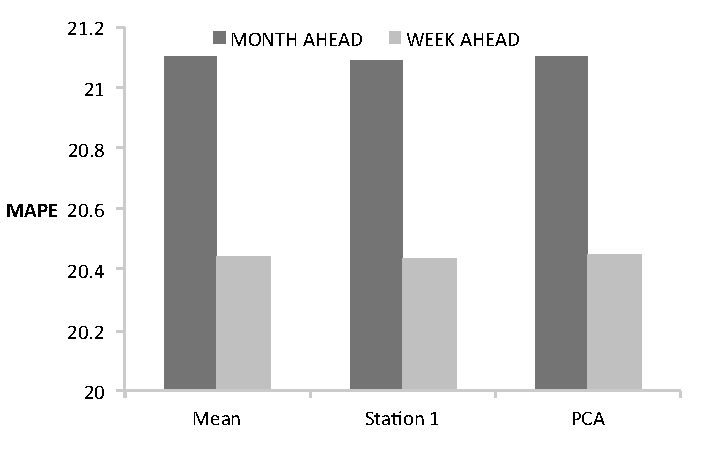
\includegraphics[width=\linewidth]{gfx/results/temp/MAPE-temp-source-effect.pdf}
\caption{MAPE and PINBALL for LM using different temperature inputs as feature. The other features are the type of day, the hour, time of year and the two lag variables.}
\label{fig:load-temp-source}
\end{figure}
%Model temperature by hour

\subsubsection{Predicting Temperature for Load Training Period}
Concerned that training the load models on the true temperature and then performing forecasts using the rather inaccurate temperature forecasts has adverse effects, we predict the temperature also for the training period of the load starting on 10/01/2006 and ending on 10/01/2010.
\begin{figure}[!ht]
\centering
\begin{subfigure}[b]{\linewidth}
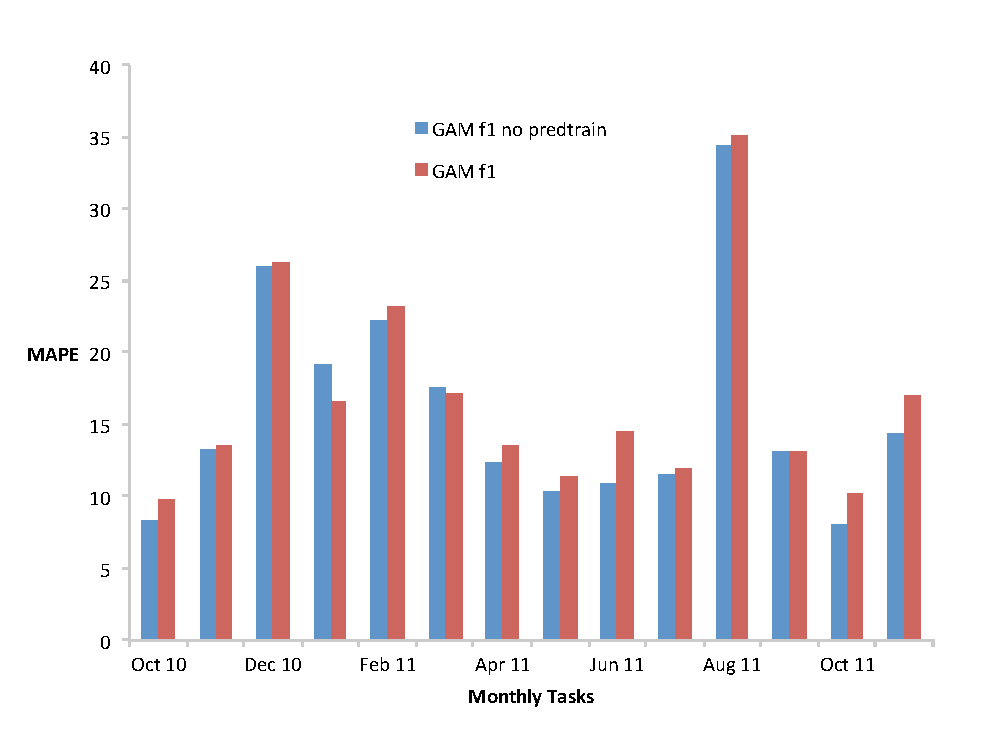
\includegraphics[width=\linewidth]{gfx/results/load/GAM-MAPE-predtrain.pdf}
\label{subfig:acf-temp-1year}
\end{subfigure}
\begin{subfigure}[b]{\linewidth}
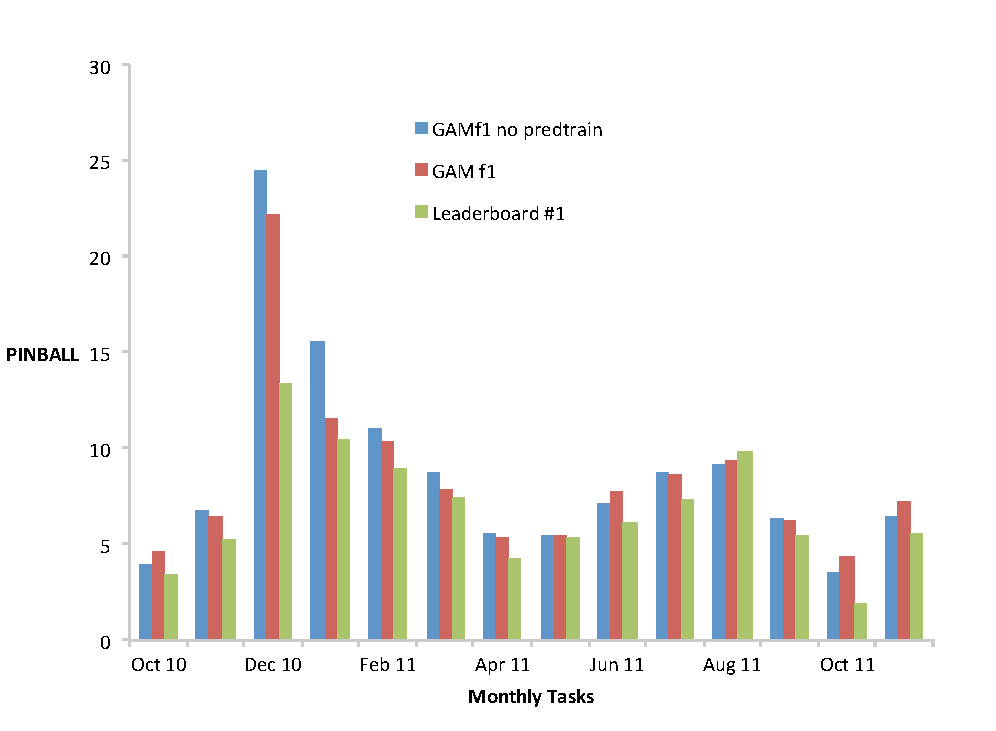
\includegraphics[width=\linewidth]{gfx/results/load/GAM-PINBALL-predtrain.pdf}
\label{subfig:acf-load-1year}
\end{subfigure}
\caption{MAPE and PINBALL scores for different temp models.}
\label{fig:load-predtrain}
\end{figure}
On average the MAPE score increases with predicting the temperature for the load training period (\textbf{predtrain}) (Figure \ref{fig:load-predtrain}), however, the pinball error decreases. This is not only true for the GAM model depicted, but also for different configurations of the other forecasting methods mentioned.
% why? answer this in the presentation
\begin{comment}
\begin{figure}[!ht]
\centering
\begin{subfigure}[b]{\linewidth}
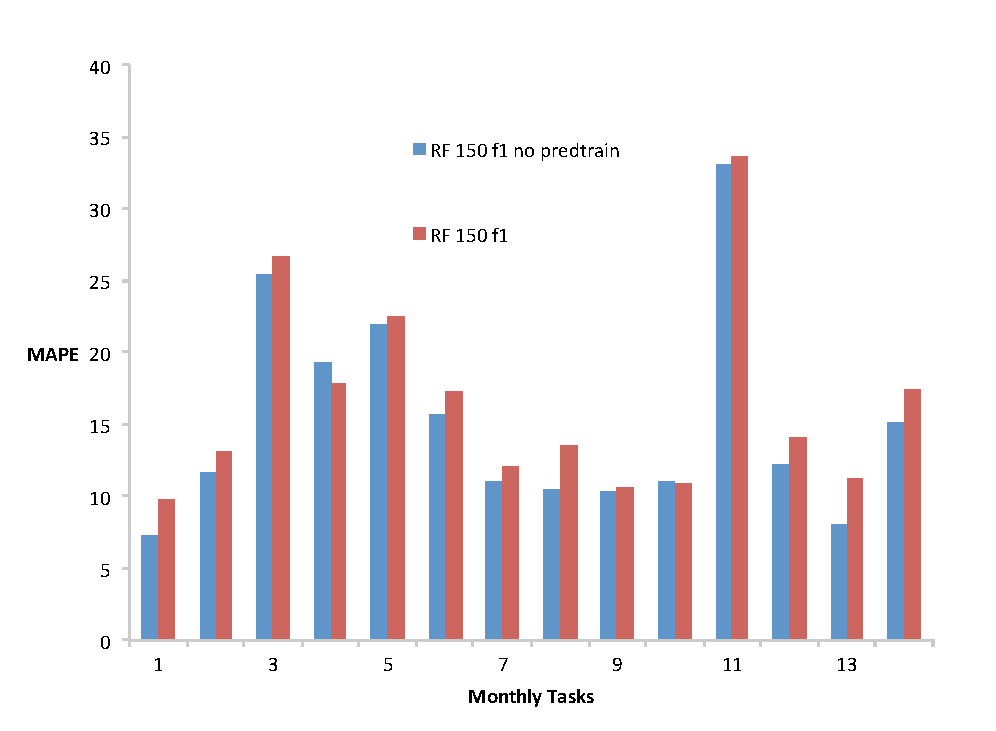
\includegraphics[width=\linewidth]{gfx/results/load/RF-150-GAMF1-MAPE-predtrain.pdf}
\label{subfig:acf-load-1year}
\end{subfigure}
\begin{subfigure}[b]{\linewidth}
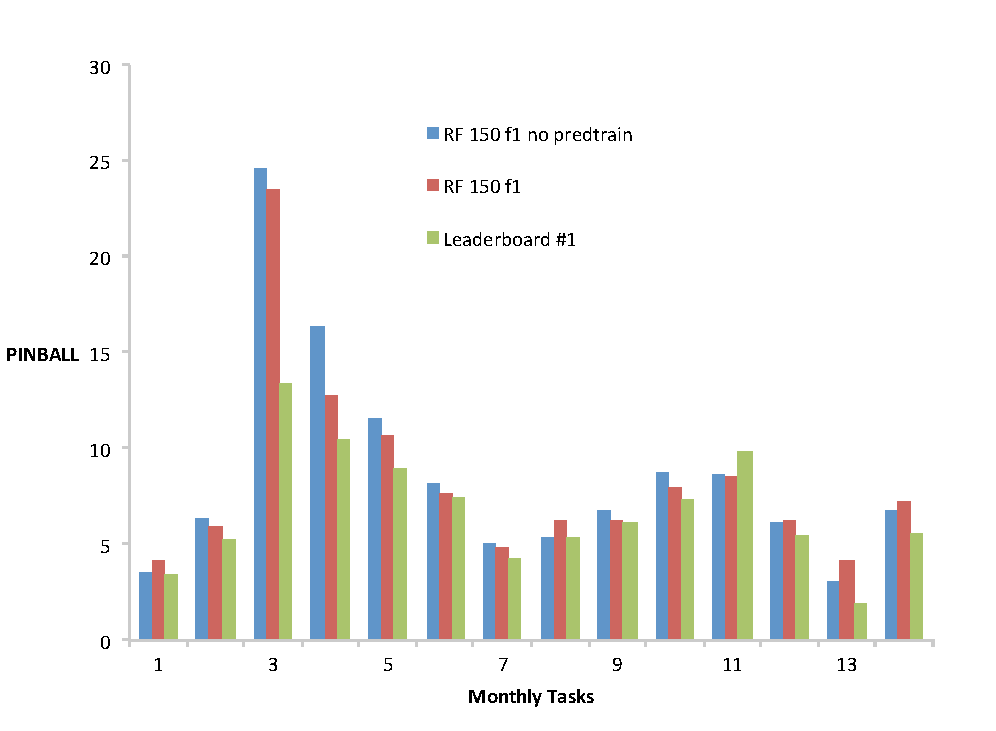
\includegraphics[width=\linewidth]{gfx/results/load/RF-150-GAMF1-PINBALL-predtrain.pdf}
\label{subfig:acf-load-1year}
\end{subfigure}
\caption{MAPE and PINBALL scores for different temp models.}
\label{fig:load-predtrain}
\end{figure}
\end{comment}

\subsubsection{Effect of the Time Horizon}
In section \ref{sec:time-lags} we demonstrated the periodicity the serial correlation of the load data possesses. Using this characteristic we would like to improve the forecasts by predicting the first or only 4 weeks of the time horizon of a month, allowing us to use more recent lagged load values. Figure \ref{fig:load-weeks} shows how the MAPE and pinball evolve by week of a month that is to be predicted on average. We show two plots, one for a random forest model and one for a GAM model. These plots show that the errors are lower for the first weeks compared to the 4th week. For the effect the change of the time horizon has compared to the month ahead prediction please consult Figure \ref{fig:load-final}. 
\begin{figure}[!ht]
\centering
\begin{subfigure}[b]{.49\linewidth}
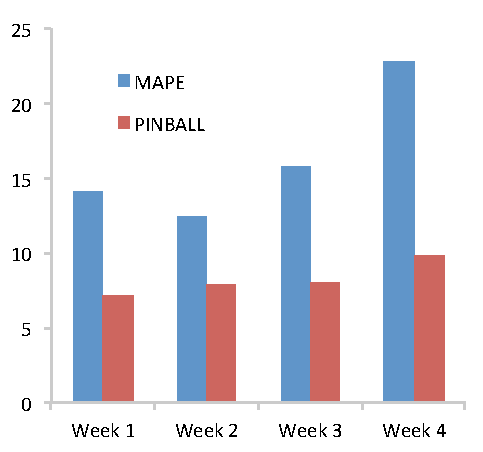
\includegraphics[width=\linewidth]{gfx/results/load/LOAD-WEEKS-MAPE-PINBALL.pdf}
\caption{RF tree 100 model with yearly and recent lagged values.}
\label{subfig:acf-temp-1year}
\end{subfigure}
\begin{subfigure}[b]{.49\linewidth}
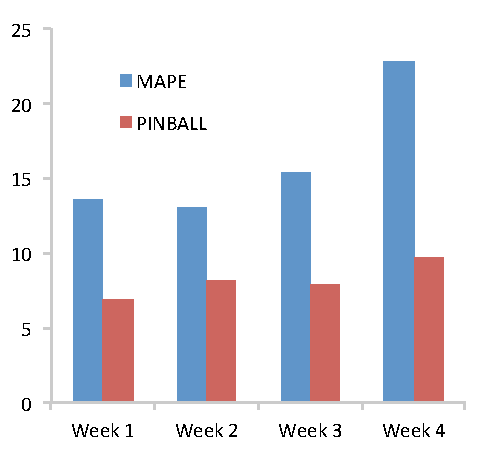
\includegraphics[width=\linewidth]{gfx/results/load/LOAD-WEEKS-MAPE-PINBALL-GAM.pdf}
\caption{GAM formula 5 with yearly and recent lagged values.}
\label{subfig:acf-load-1year}
\end{subfigure}
\caption{Scores by week 1-4 averaged over the monthly tasks making up the forecasting horizon.}
\label{fig:load-weeks}
\end{figure}
The simulation results suggest overall that the inclusion of a recent lag variable on top of a lagged value of 365 days has a positive effect on the model performace. Figure \ref{fig:load-DLAG} shows both MAPE and pinball in separate plots for two GAM models with week ahead forecasting horizon including and excluding recent lagged values. However, it has to be noted that the overall improvement for both GAM and random forest models is around 0.1 for MAPE and even less for the pinball score.
%set the basis by plotting MAPE \& PINBALL scores by week over w1, w2, w3, w4; one curve for every month in CV\\
%do this for every method\\
%as well as a comparison of the best performing configuration of every method among each other\\
\begin{figure}[!ht]
\centering
\begin{subfigure}[b]{\linewidth}
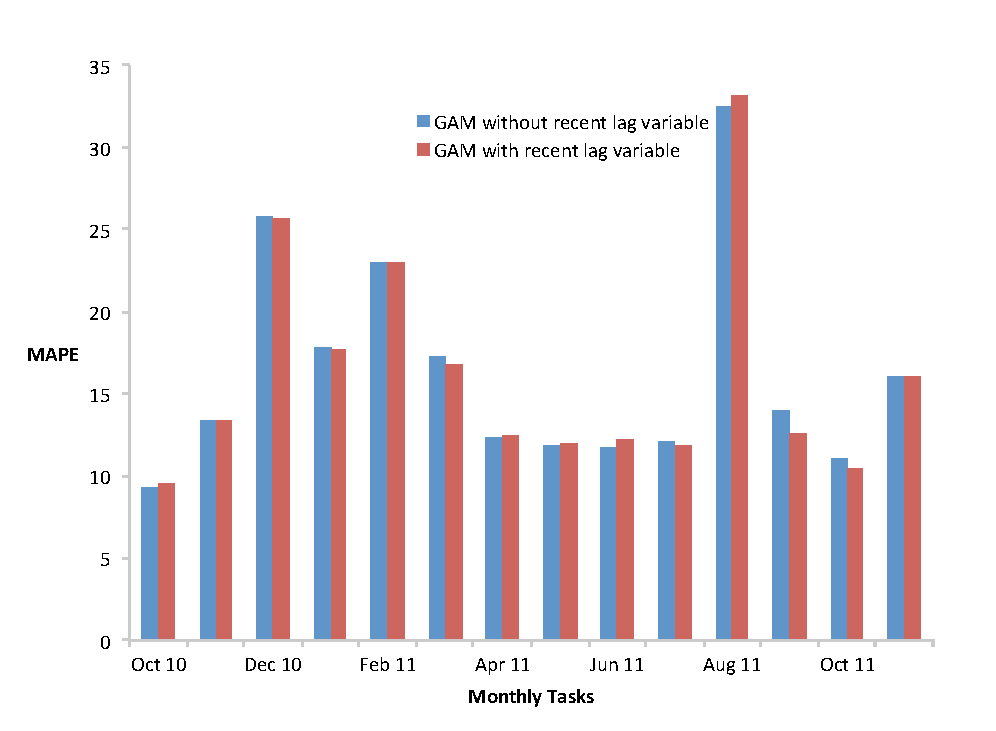
\includegraphics[width=\linewidth]{gfx/results/load/GAM-MAPE-DLAG.pdf}
\label{subfig:DLAG1}
\end{subfigure}
\begin{subfigure}[b]{\linewidth}
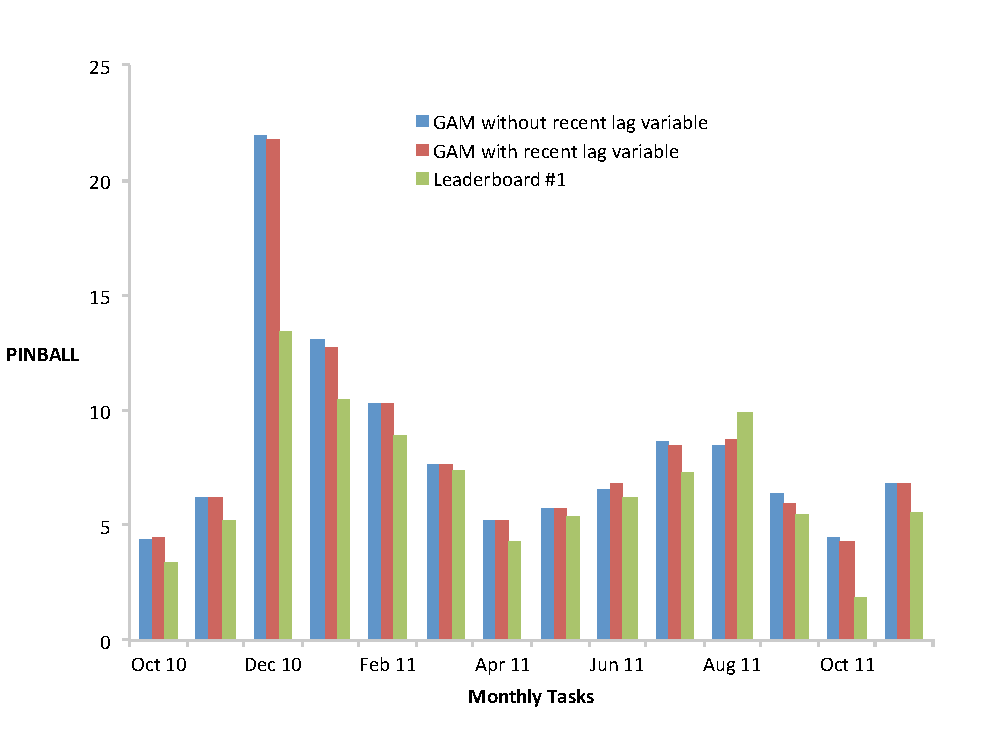
\includegraphics[width=\linewidth]{gfx/results/load/GAM-PINBALL-DLAG.pdf}
\label{subfig:DLAG2}
\end{subfigure}
\caption{MAPE and Pinball scores on monthly tasks for GAM models with and without recent lagged values. The temperature model used is the GAM f1 model shown in \ref{fig:temp-results}}
\label{fig:load-DLAG}
\end{figure}

\subsubsection{Effect of different Daytype Assignments}
After having dealt with the lag variables, we briefly address the different assignments of day types. Figure \ref{fig:load-DAYT} shows that the different assignments have practically no effect on the MAPE and pinball when implemented in different GAM models. This makes sense because when probing the data no weekday versus weekend patterns or patterns for federal holidays seem to catch the eye. The load data provided is that of one utility and there is no information as to the proportion of domestic to industrial consumption. In other words: we have no clue as to where exactly the energy is from and what it is used for, rendering analysis in this respect difficult. 
\begin{figure}[!ht]
\centering
\begin{subfigure}[b]{\linewidth}
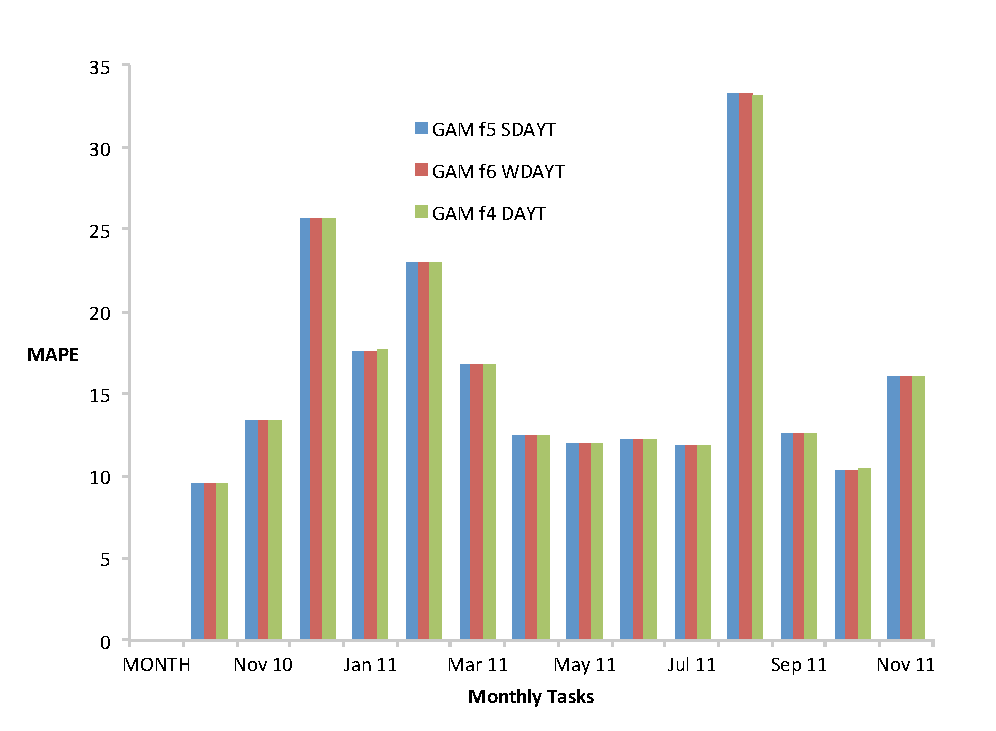
\includegraphics[width=\linewidth]{gfx/results/load/DAYT-MAPE.pdf}
\label{subfig:acf-temp-1year}
\end{subfigure}
\begin{subfigure}[b]{\linewidth}
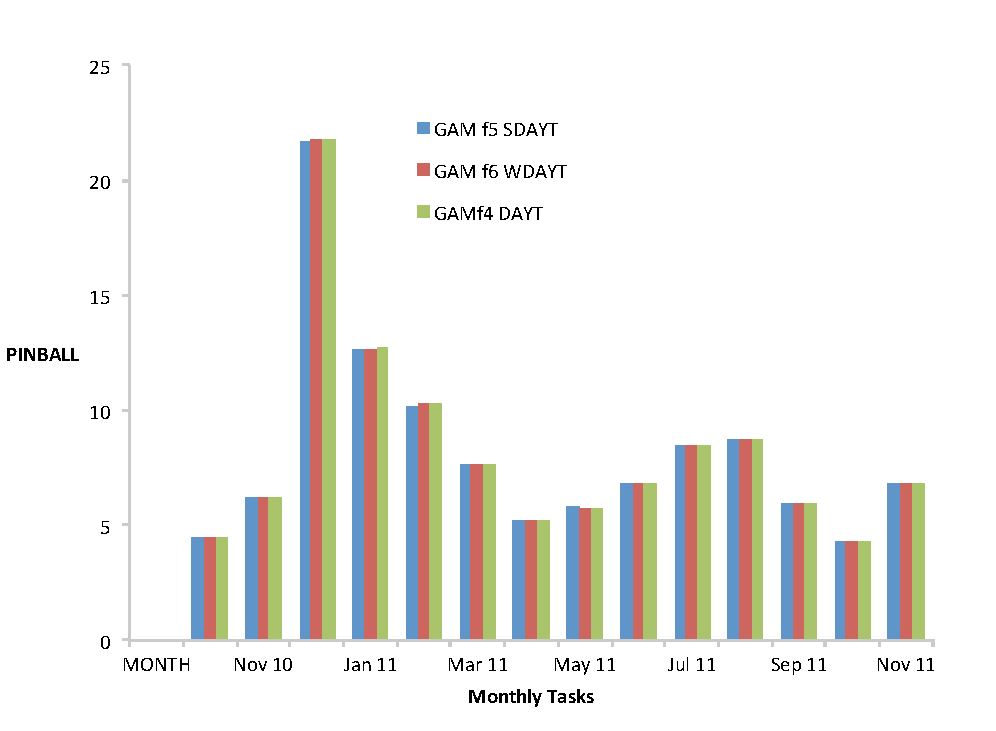
\includegraphics[width=\linewidth]{gfx/results/load/DAYT-PINBALL.pdf}
\label{subfig:acf-load-1year}
\end{subfigure}
\caption{MAPE and PINBALL scores for different GAM models with monthly forecasting.}
\label{fig:load-DAYT}
\end{figure}

\subsubsection{Best Performancing Method Configuration}
The best results obtained after simulating a large number of temperature and load forecast combinations and method configurations are for a random forest model with 100 trees (no daytype, week ahead forecasting, prediction of temperature for load training) using a neural network with 15 hidden units for the temperature forecast (1 month forecast horizon). The average for the entire evaluation period MAPE and pinball scores are 16.094 and 7.999 respectively. Using the pinball errors displayed in figure \ref{subfig:final-pinball} we can now compute a hypothetical position on the final leaderboard of the GEFCom2014 competition using the mentioned model configuration. The rules state: ``The final score is the trimmed mean of the weekly scores. The highest and lowest weekly scores are discarded. The participants are required to submit entries for at least 9 out of 12 weeks during the scoring period to be eligible for a position in the final leaderboard.'' Excluding the first three months (Oct, Nov, Dec) that were the trial period and the last month for which the real data has not been published, we can compute the trimmed mean excluding the best and worst pinball scores of 11 tasks. The hypothetical score thus is \textbf{7.16}. This score would have resulted in a third place on the final leaderboard, beaten by 6.93 (\#1) and 7.10 (\#2). The positions on the scoreboards for the individual tasks are displayed in figure \ref{subfig:task-pos} comparing the different prediction horizons. The average position for the task leaderboards would be 5.64. However, not every contestant reached a position equally high up the scoreboard every week allowing for our improved hypothetical position on the final leaderboard.
\begin{figure}[!ht]
\centering
\begin{subfigure}[b]{\linewidth}
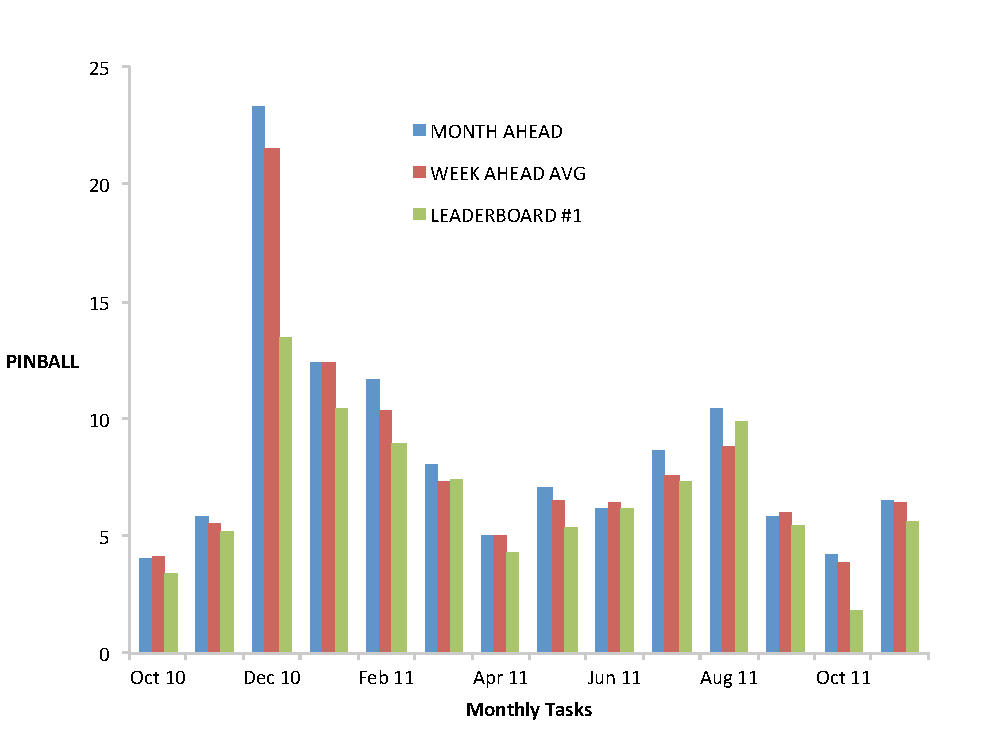
\includegraphics[width=\linewidth]{gfx/results/load/LOAD-BEST-PINBALL.pdf}
\caption{RF 100 ntrees: pinball scores compared to \#1 position on task scoreboard.}
\label{subfig:final-pinball}
\end{subfigure}
\begin{subfigure}[b]{\linewidth}
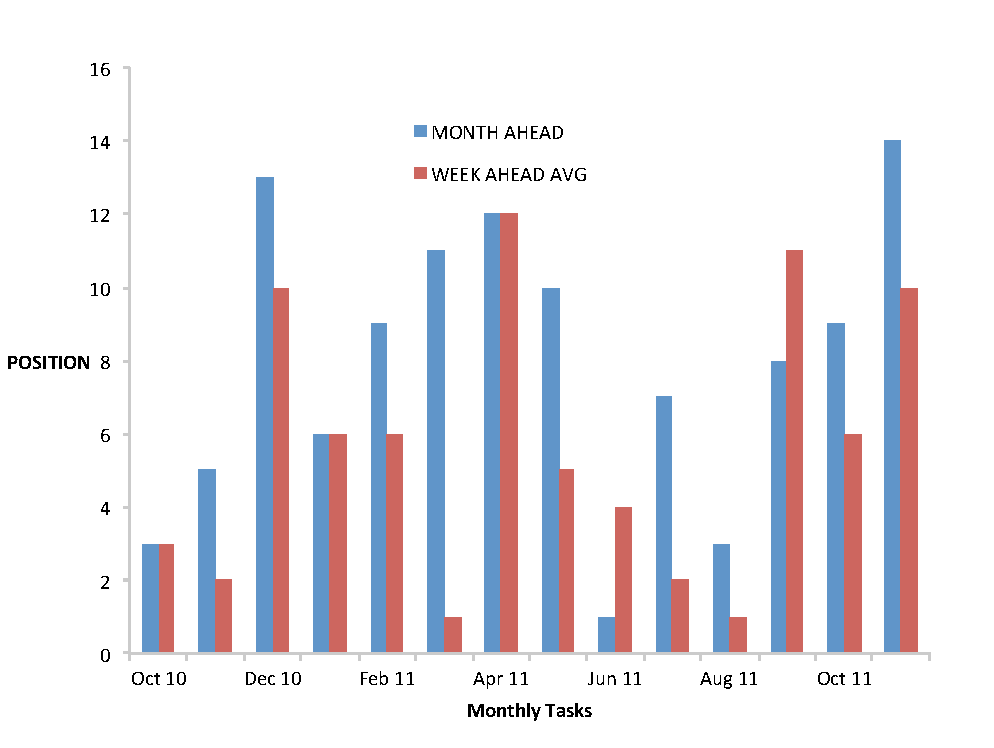
\includegraphics[width=\linewidth]{gfx/results/load/LOAD-BEST-POSITION.pdf}
\caption{RF 100 ntrees: individual task scoreboard positions}
\label{subfig:task-pos}
\end{subfigure}
\caption{Pinball and hypothetical positions for the individual tasks (including trials Oct - Dec 2010) for a random forest with 100 trees. The model does not use a day type, yet does include a variable for recent lags. The method use for the temperature prediction is a neural network with month ahead forecasting.}
\label{fig:load-final}
\end{figure}

\section{Conclusion}
% calculation of actual score would have depended on submissions
In this report we show that competitive scores with respect to the GEFCom 2014 leaderboard can be achieved using relatively simple models. Computing competition scores in hindsight is not the ``real deal'', however, since the student started with little knowledge of forecasting methodologies it is motivating to see what is achievable. The results are striking, because more time was spent on defining different combinations of smoothing functions for the GAM models than on any on either the neural network or the random forest models. However, these methods performed best on temperature and load forecasting respectively. All that was needed was to set the \textbf{ntrees} parameter or hidden units parameter and plugin a group of features. Grid search on the \textbf{ntrees} parameter may yield an optimal chosing in between the values 50, 100, 150 that were specified for load forecasting. Preferable about the generalized additive model is that it allows for relationships to be defined by the user, which are then either validated or not through training a model. This gives it more explanarotary power than running a more ``blackbox'' method like a neural network or random forest.\\
The results are by no means perfect, much can surely still be improved with deeper data exploration and more time dedicated to the study of papers and theory of the forecasting methods that were used. A next stop could be to combine the GAM and random forest models to produce ensemble forecasts and evaluate these. Further, residual analysis may uncover patterns in the data. The student needed quite some time to get acquainted with the forecasting workflow and the problem of having two linked forecasting tasks, so having a working pipeline was the priority.\par
In summary, the project has been very enriching since the student knew hardly anything about the forecasting workflow before the commencement of this project and feels he has been given a good introduction to the subject. The student would like to sincerely thank Tri Wijaya and Matteo Vasirani for sharing their knowledge and valuable time.

\bibliographystyle{IEEEtran}
\bibliography{references}{}

\end{document}


